\documentclass[11pt,a4paper,english]{article}
\usepackage[titletoc, title]{appendix}
\usepackage{amsmath}
\usepackage{amssymb}
\usepackage{bm}
\usepackage{array}
\usepackage{babel}
\usepackage{bbding}
\usepackage{color}
\usepackage[normal]{caption}
\usepackage{subcaption}
\usepackage{epsfig}
\usepackage{graphicx}
\usepackage{pdflscape}
\usepackage{lipsum}
%\usepackage{multirow}
\usepackage{psfrag}
\usepackage{proofapnd}
\usepackage[round]{natbib}
%\usepackage{bbm}
%\usepackage[T1]{fontenc}
%\usepackage[normal]{caption2} % for caption
\usepackage{rotating}
\usepackage[margin=2cm]{geometry} % for the same margin
\usepackage{latexsym}
%\usepackage{subfig}
\usepackage{setspace}
\usepackage{slashbox}
\usepackage{enumitem}
\usepackage{booktabs}
\usepackage{tabularx}
\usepackage{longtable,booktabs}
\usepackage{authblk}
\usepackage{hyperref}
\usepackage{indentfirst} % Macht eine Einrückung nach der Section
\bibliographystyle{ecta}
\usepackage{tabularx}


\definecolor{markergreen}{rgb}{0.6, 1.0, 0}
\definecolor{darkgreen}{rgb}{0, .5, 0}
\definecolor{darkorange}{rgb}{1,0.3,0}
\definecolor{darkred}{RGB}{.7,0,0}
\definecolor{darkblue}{RGB}{0,29,245}
\definecolor{orange}{RGB}{239, 133, 54}
\definecolor{lightblue}{RGB}{59, 188, 175}

\providecommand{\marker}[1]{\fcolorbox{markergreen}{markergreen}{{#1}}}
\providecommand{\mj}[1]{\textcolor{darkred}{#1}}
\providecommand{\francis}[1]{\textcolor{darkgreen}{#1}}
\providecommand{\natp}[1]{\textcolor{darkorange}{#1}}

\setlist[itemize]{leftmargin=*}
\setlist[description]{leftmargin=*}

%\setlength{\topmargin}{0.0 in} \setlength{\textwidth}{6in}
%\setlength{\oddsidemargin}{0.5in}
%\setlength{\evensidemargin}{-0.01in} \setlength{\textheight}{9in}
\captionsetup{font={onehalfspacing,small}, labelfont=bf}

\title{\LARGE \bf Hedging Cryptos with Bitcoin Futures.}
%\title{\natp{\large\bf Copula-based hedging of cryptocurrencies with Bitcoin futures}}
\author{
%	\begin{tabular}[t]{ccc}
        \and
        Francis Liu\thanks{
			Department of Business and Economics, Berlin School of Economics and Law, Badensche Str. 52, 10825 Berlin, Germany.
            Blockchain Research Center, Humboldt-Universität zu Berlin, Germany.
            International Research Training Group
1792, Humboldt-Universität zu Berlin, Germany.
     E-mail: \texttt{Francis.Liu@hwr-berlin.de}.}
        \and
		Meng-Jou Lu
        \thanks{
             Department of Finance, Asia University, 500, Lioufeng Rd., Wufeng, Taichung 41354, Taiwan
             Department of Finance, Asia University, 500, Lioufeng Rd., Wufeng, Taichung 41354, Taiwan
     E-mail: \texttt{mangrou@gmail.com}.}
		 \and
        Natalie Packham\thanks{
			Department of Business and Economics, Berlin School of Economics and Law, Badensche Str. 52, 10825 Berlin, Germany.
            International Research Training Group 1792, Humboldt-Universität zu Berlin, Germany.
     E-mail: \texttt{packham@hwr-berlin.de}.}
		 \and
         Wolfgang Karl H\"ardle\thanks{
			Blockchain Research Center, Humboldt-Universit\"at zu Berlin, Germany. Wang Yanan Institute for Studies in Economics, Xiamen University, China. Sim Kee Boon Institute for Financial Economics, Singapore Management University, Singapore. Faculty of Mathematics and Physics, Charles University, Czech Republic. National Chiao Tung University, Taiwan.
     E-mail: \texttt{haerdle@wiwi.hu-berlin.de}.}
        \thanks{ Financial support of the European Union's Horizon 2020 research and innovation program ``FIN-TECH: A Financial supervision and Technology compliance training programme" under the grant agreement No 825215 (Topic: ICT-35-2018, Type of action: CSA), the European Cooperation in Science \& Technology COST Action grant CA19130 - Fintech and Artificial Intelligence in Finance - Towards a transparent financial industry, the Deutsche Forschungsgemeinschaft's IRTG 1792 grant, the Yushan Scholar Program of Taiwan, the Czech Science Foundation's grant no. 19-28231X / CAS: XDA 23020303, as well as support by Ansar Aynetdinov (\texttt{ansar.aynetdinov@hu-berlin.de}) are greatly acknowledged.
     }
%	\end{tabular}
}
\date{This version: \today}
%%%%%%%%%%%%%%%%%%%%%%%%%%%%%%%%%%%%%%%%%%%%%%%%%%%%%%%%%%%%%%%%%%%%%%%%%%%%%%%%%%%%%%%%%%%%%%%%
\renewcommand{\baselinestretch}{1.2}
%\newcommand{\indicator}{$1{\hskip -2.5 pt}\hbox{I}$}
\newcommand{\indicator}{I}
%%
%% $Id: Definitions.tex,v 1.6 2008/07/26 14:55:50 natalie Exp $
%% $Source: /Users/natalie/cvs/tex/dynamics/Definitions.tex,v $
%% $Date: 2008/07/26 14:55:50 $
%% $Revision: 1.6 $
%%

%\usepackage{mathrsfs}

%% GENERAL DEFINITIONS
\unitlength1cm

%% COMMAND DEFINITIONS
\newcommand{\E}{{\mathbb{E}}}
%%\renewcommand{\E}{{\mathds E}}
%%\renewcommand{\E}{{\varmathbb{E}}}
%%\renewcommand{\E}{{\mathrm{I\!E}}}
\providecommand{\R}{{\mathbb{R}}}
\newcommand{\T}{{\mathbb{T}}}
\newcommand{\Fb}{{\mathbb{F}}}
\newcommand{\Eqn}{{\mathbb{E}}_{{\bf Q}_N}}
\newcommand{\Eq}{{\mathbb{E}}_{{\bf Q}}}
\newcommand{\Eqm}{{\mathbb{E}}_{{\bf Q}_M}}
\newcommand{\EqT}{{\mathbb{E}}_{{\bf Q}_T}}
\newcommand{\EqTz}{{\mathbb{E}}_{{\bf Q}_{T_2}}}
\newcommand{\EqTe}{{\mathbb{E}}_{{\bf Q}_{T_1}}}
\newcommand{\EqSe}{{\mathbb{E}}_{{\bf Q}_{S^1}}}
\newcommand{\EqSz}{{\mathbb{E}}_{{\bf Q}_{S^2}}}
\newcommand{\p}{{\bf P}}
%%\renewcommand{\p}{{\mathds{P}}}
%%\renewcommand{\p}{{\varmathbb{P}}}
%%\renewcommand{\p}{{\mathrm{I\!P}}}
\newcommand{\pas}{\text{{\bf P}--a.s.}}
\newcommand{\paa}{\text{{\bf P}--a.a.}}
\newcommand{\qas}{\text{{\bf Q}--a.s.}}
\newcommand{\e}{{\bf e}}
\newcommand{\q}{{\bf Q}}
\newcommand{\qn}{{\bf Q}_N}
\newcommand{\qm}{{\bf Q}_M}
\newcommand{\qT}{{\bf Q}_T}
\newcommand{\qTz}{{\bf Q}_{T_2}}
\newcommand{\qTe}{{\bf Q}_{T_1}}
\newcommand{\qS}{{\bf Q}_S}
\newcommand{\qSe}{{\bf Q}_{S^1}}
\newcommand{\qSz}{{\bf Q}_{S^2}}
\newcommand{\F}{{\cal F}}
\newcommand{\G}{{\cal G}}
\newcommand{\A}{{\cal A}}
\newcommand{\Hc}{{\cal H}}
\newcommand{\dP}{{\rm d}{\bf P}}
\newcommand{\du}{{\rm d}u}
%%\newcommand{\dt}{{\rm d}t}
\newcommand{\dd}{{\rm d}}
\newcommand{\df}{{\rm \bf DF}}
\providecommand{\N}{{\mathbb N}}
\providecommand{\Ncdf}{{\rm N}}
%\renewcommand{\Ncdf}{{\Phi}}
\newcommand{\n}{{\rm n}}
\newcommand{\emb}{\bf \em}
\newcommand{\1}{\textbf{1}}
\newcommand{\qs}{{\q_{\rm Swap}}}
\newcommand{\fx}{{\rm fx}}
\newcommand{\V}{{\rm Var}}
%\newcommand{\C}{{\bf C}}
\newcommand{\Om}{{\Omega}}
\providecommand{\limn}{\ensuremath{\lim_{n\rightarrow\infty}}}
\providecommand{\qv}[2]{\ensuremath{\langle #1,#1\rangle_{#2}}}

%% ENVIRONMENT DEFINITIONS
%\newtheorem{prop}{Proposition}[section]
%\newtheorem{theo}{Theorem}[section]
%\newtheorem{lem}{Lemma}[section]
%\newtheorem{ass}{Assumption}[section]
%\newtheorem{cor}{Corollary}[section]
%\newtheorem{aufg}{Exercise}[section]
%\newtheorem{defi}{Definition}[section]

\ifx\prop\undefined
\newtheorem{prop}{Proposition}[section]
\fi
\newtheorem{theo}[prop]{Theorem}
\newtheorem{lem}[prop]{Lemma}
\newtheorem{cor}[prop]{Corollary}
\newtheorem{defi}[prop]{Definition}

%% enumeration in lists
\providecommand{\labelenumi}{{\rm (\roman{enumi})}}
   %\setlength{\topsep}{0cm}
    \setlength{\labelsep}{0.3cm}
    %\setlength{\itemindent}{0cm}
   \setlength{\leftmargin}{10cm}
    \setlength{\labelwidth}{5cm}

\providecommand{\cadlag}{c\`adl\`ag }
\providecommand{\cadlagns}{c\`adl\`ag}
\providecommand{\caglad}{c\`agl\`ad }
\providecommand{\cad}{c\`ad}
\providecommand{\cag}{c\`ag}
\providecommand{\levy}{L\'evy\ }
\providecommand{\levyns}{L\'evy}
\providecommand{\levyito}{L\'evy-It\^o\ } 
\providecommand{\levykhinchin}{L\'evy-Khinchin\ }
\providecommand{\D}{\ensuremath{D(\R_+,\R)}}
\providecommand{\Dsig}{\ensuremath{D(\R_+, \R_+\setminus\{0\}})}
\providecommand{\Dd}{\ensuremath{D(\R_+,\R^d)}}
\providecommand{\C}{\ensuremath{C(\R_+,\R)}}
\providecommand{\Cd}{\ensuremath{C(\R_+,\R^d)}}
\providecommand{\rpos}{\ensuremath{{[0,\infty)}}}

\def\Z{{\mathbb Z}}
%\def\N{{\mathbb N}}
%\def\R{{\mathbb R}}
%\def\C{{\mathbb C}}
%\def\H{{\mathbb H}}
\def\P{{\mathbb P}}
\def\Q{{\mathbb Q}}
%\def\E{{\mathbb E}}
\def\I{{\mathbb I}}
%\def\T{{\mathbb T}}
%\def\F{{\mathbb F}}
\def\M{{\mathbb M}}
%\def\Hc{{\mathcal H}}
\def\Mc{{\mathcal M}}
\def\filtration#1{{\ensuremath\mathcal{#1}}}
%\def\filt{{\mathcal F}}
\def\tp{\tilde{\p}}
\providecommand{\vec}[1]{\ensuremath{\bm #1}}
\providecommand{\vecb}[1]{\ensuremath{\bm #1}}
\providecommand{\abs}[1]{\ensuremath{\lvert#1\rvert}}
\providecommand{\norm}[1]{\ensuremath{\lVert#1\rVert}}
\providecommand{\var}{\ensuremath{\text{Var}}}
\providecommand{\cov}{\ensuremath{\text{Cov}}}
\providecommand{\borel}[0]{\ensuremath{\mathcal{B}}}
\providecommand{\intinf}[0]{\ensuremath{\int_{-\infty}^\infty}}
\providecommand{\intpos}[0]{\ensuremath{\int_0^\infty}}
\providecommand{\intneg}[0]{\ensuremath{\int_{-\infty}^0}}
\providecommand{\todo}[1]{\footnote{#1}}
\providecommand{\dynkin}[0]{\ensuremath{\mathcal D}}
\providecommand{\ce}[2]{\ensuremath{\E(#1|\filtration{#2})}}
\providecommand{\inv}[1]{\ensuremath{#1^{(-1)}}}
\providecommand{\os}[2]{\ensuremath{#1^{(#2)}}}
\providecommand{\pos}[2]{\ensuremath{h_{#1}(#2)}}
%\providecommand{\poslong}[2]{\ensuremath{h(#1, #2)}}
\providecommand{\poslong}[3]{\ensuremath{h_{#1, #2}(#3)}}

%% Class of finite variation processes
\providecommand{\classfv}{\ensuremath{\mathscr V}}
\providecommand{\classv}{\ensuremath{\mathscr V}}
%% Stochastic integral operator
\providecommand{\stint}{\ensuremath{\cdotp}}
\providecommand{\classh}{\ensuremath{\mathscr H^2}}
\providecommand{\classhloc}{\ensuremath{\mathscr H^2_{\rm loc}}}
\providecommand{\classm}{\ensuremath{\mathscr M}}
\providecommand{\classmloc}{\ensuremath{\mathscr M_{\rm loc}}}
\providecommand{\classl}{\ensuremath{L^2}}
\providecommand{\classlloc}{\ensuremath{L^2_{\rm loc}}}
\providecommand{\classa}{\ensuremath{\mathscr A}}
\providecommand{\classaloc}{\ensuremath{\mathscr A_{\rm loc}}}
\providecommand{\classalocpos}{\ensuremath{\mathscr A_{\rm loc}^+}}
\providecommand{\classp}{\ensuremath{\mathscr P}}
\providecommand{\classo}{\ensuremath{\mathscr O}}
\providecommand{\classs}{\ensuremath{\mathscr S}}
\providecommand{\classsp}{\ensuremath{\mathscr S_p}}
\providecommand{\nullset}{\ensuremath{\mathscr N}}

\providecommand{\ito}{It\^o }
\providecommand{\itos}{It\^o's\, }

\providecommand{\variation}[2]{\ensuremath{\rm V_{#1}(#2)}}
\renewcommand{\H}{\ensuremath{\mathcal H}}
%% CPO distribution
\providecommand{\cpo}{\ensuremath{{\rm CPO}}}
\providecommand{\Fsigma}{\ensuremath{\mathcal \F_\infty^\sigma}}
\providecommand{\sigd}{\ensuremath{\mathscr D}}

%% Credit spreads
\providecommand{\s}{{\bf s}}
\providecommand{\classu}{\ensuremath{\mathscr U}}

\providecommand{\sX}{\ensuremath{\mathcal X}}
\providecommand{\sY}{\ensuremath{\mathcal Y}}
\providecommand{\dx}{\ensuremath{\frac{\partial}{\partial x}}} %%
\providecommand{\dt}{\ensuremath{\frac{\partial}{\partial t}}} %%
\providecommand{\dy}{\ensuremath{\frac{\partial}{\partial y}}} %%
\newcommand{\argmax}{\operatornamewithlimits{argmax}}
\newcommand{\argmin}{\operatornamewithlimits{argmin}}


\begin{document}

\newtheorem{lemma}{Lemma}
\newtheorem {proposition}[lemma]{Proposition}
\newtheorem {corollary}{Corollary}
\newtheorem {theorem}{Theorem}
\newtheorem{claim}[lemma]{Claim}
\newtheorem{comment}[lemma]{Comment}
\newtheorem{example}[lemma]{Example}
\newtheorem{fact}[lemma]{Fact}
\newtheorem{defn}[lemma]{Definition}
\newtheorem{exercise}{Exercise}[section]

\newtheorem{programming}[exercise]{Programming assignment}
\newenvironment{proof}{{\flushleft\textbf{\textsl{Proof.\ \ }}}}{\hfill{\hfill\rule{2mm}{2mm}}}
\pagenumbering{arabic}

\maketitle

%%%%%%%%%%%%%%%%%%%%%%%%%%%%%%%%%%%%%%%%%%%%%%%%%%%%%%%%%%%%%%%%%%%%%%%%%%%%%%%%%%%%%%%%%%%%%%%
\begin{abstract}
\footnotesize{
The introduction of derivatives on Bitcoin, in particular the launch of futures contracts on CME in December 2017 and introduction of cryptocurrency index (CRIX) \citep{trimborn2018crix},
enables investors to hedge risk exposures of Bitcoin by futures or cryptocurrency index.
We investigate methods of finding the optimal hedge ratio $h^*$ under different dependence structures modeled by copulae and optimality definition described by a range of risk measures.
Because of volatility swings and jumps in Bitcoin prices, the traditional variance-based approach to obtain the hedge ratios is infeasible.
The approach is therefore generalised  to various risk measures, such as Value-at-Risk, Expected Shortfall and Spectral Risk Measures,
and to different copulae for capturing the dependency between spot and future returns, such as the Gaussian, Student-$t$,
NIG and Archimedean copulae. Various measures of hedge effectiveness in out-of-sample tests give insights in the practice of hedging Bitcoin and the CRIX,
a cryptocurrency index.\\

\noindent {\bf JEL classification:}  \\
\noindent {\bf Keywords:} Portfolio Selection, Spectral Risk Measurement,  Coherent Risk}\pagestyle{empty}\\
\end{abstract}

\natp{{\bf TODO}:
  \begin{itemize}
  \item Please generate all graphics as pdf and possibly eps. pdf is a
    vector graphic format, so it scales well. eps may be
    required during the publishing process.
  \item Plackett copula: This is a bivariate copula only, which is
    probably one of the reasons it is not commonly found in finance
    applications. It does not have tail dependence, which is one of
    the things we typically look for in finance. We need a compelling
    reason why it is of interest, otherwise I suggest to remove it.
  \item We need to discuss if we use copulas or copulae. I have a
    preference for copulas, which is the terminology used by Nelsen,
    McNeil et al., Joe.
  \item The introduction needs to be revised, see comments
    below. Think about what needs to go into the introduction and what
    does not, and then stick to this in a concise way. Also, re-read
    every sentence 2-3 times and think carefully about what it says
    and what it is supposed to say. 
  \end{itemize}
}

%\tableofcontents

\clearpage
%%%%%%%%%%%%%%%%%%%%%%%%%%%%%%%%%%%%%%%%%%%%%%%%%%%%%%%%%%%%%%%%%%%%%%%%%%%%%%%%%%%%%%%%%%%%%%%%%%%%%%%%%%%%%%%%%%%%%%%%%%%%%%%%%%%%%%%%%%%%%%%%%%%%%%
%%%%%%%%%%%%%%%%%%%%%%%%%%%%%%%%%%%%%%%%%%%%%%%%%%%%%%%%%%%%%%%%%%%%%%%%%%%%%%%%%%%%%%%%%%%%%%%%%%%%%%%%%%%%%%%%%%%%%%%%%%%%%%%%%%%%%%%%%%%%%%%%%%%%%%
\section{Introduction}\label{sec:introduction}

Cryptocurrencies (CCs) are a growing asset class.
Many more CCs are now available on the market since the first
cryptocurrency Bitcoin (BTC) was introduced by
\citet{nakamoto2019bitcoin}. \natp{\em [BTC was introduced in 2009.]}
In response to the rapid development of the cryptocurrency market, CRIX \citep{trimborn2018crix} is developed to represent the whole
market by an index aggregating the price of important coins in the
market. \natp{\em [Not necessary to mention CRIX here, let's speak
  about what the paper is about.]}
In Dec 2017, the CME group launched its new bitcoin future contract.
While more and more investors (individuals and institution) are adding
CCs and their derivatives into their \natp{portfolios (was: portfolios)},
we see the need to understand the downside risk and find a suitable way to hedge.
We are particularly interested in resisting extreme risks and improve their profits.
In this paper, we investigate the performance of different copulae and
risk measures in hedging Bitcoin and CRIX with Bitcoin
futures. \natp{\em [$\leftarrow$ Make this the first sentence of the paper!]}
Copulas provide the flexibility to model multivariate random variable
separately by its margins and dependence structure. 
Different risk measures accounts for investors' risk attitude.
Vast literature discussed the relationship between risk measures and investor's risk attitude, we refer readers to
\citet{artzner1999coherent} for an axiomatic, economic reasoning approach of risk measure construction;
\citet{embrechts2002correlation} for reasoning of using Expected Shortfall and Spectral Risk in addition to VaR;
\citet{Acerbi2002} for direct linkage between risk measures and investor's risk attitude using the concept of "risk aversion function".
In addition to the development of risk measures, financial data is known to be non Gaussian \natp{\cite{Cont2001}}, let
alone the violate cryptocurrencies. \natp{\em [non-Gaussian is not
  very specific, a uniform r.v.\ is also non-Gaussian. Try to express
  this in a more meaningful way, e.g.\ Financial data are known to
  exhibit more extreme events than a normal distribution can capture.]}
One cannot rely on only 2nd order moment calculations in order to
minimize downside risk. \natp{\em [Why can one not rely on 2nd order
  moment calculations? This: Variance as a risk measure applies only
  to investors with certain utility functions. We know that investors'
  risk aversion is different from this, e.g.\ investors are tail-risk
  averse, etc. Add more detail and references.]}
One may turn to VaR to monitor The VaR as a sole risk measure has two disadvantages.
First, it reflects only tail probability and not tail loss, and next it is not coherent;
Coherency is a very natural property that suggest diversification will
reduce risk. \natp{\em [This needs not go in the introduction. Just
  briefly mention the risk measures, and possibly that ES and SRM are
  chosen because of their coherence.]}
\medskip

\natp{The introduction should go along the lines:
  \begin{itemize}
  \item 1-2 sentence: Which problem is solved in this paper?
  \item Background Bitcoin: Growth, but roller-coaster ride, institutional investment,
    exchange-traded futures (the exchange is important!) (5 sentences,
    with references!)
  \item Significant tail risks and basis risk lead to the need to
    investigate even static hedges (=futures) with more refined
    methods than minimum-variance based (reference to Ederington
    here; this uses variance as risk measure and correlation as
    dependence measure).
  \item To capture empirical properties, extend to other risk measures
    and dependence models. 
  \end{itemize}
  }

This paper considers a hedging problem of Bitcoin using its future and an aggregated index of cryptocurrencies CRIX,
i.e. to find an optimal hedge ratio $h^*$ such that the risk of a hedged portfolio $R^h = R^S - h^*R^F$ has
minimal risk.
We denote $R^S$ as the log return of Bitcoin spot price, $R^F$ as log return of Bitcoin future and CRIX.
The non Gaussianity and development of risk measures lead us to deploy copulae together with various risk measures as loss function to optimize the hedge ratio.
In this paper, we calibrate the log returns of Bitcoin, CRIX, and CME future by copulae,
then find the optimal quantity of assets in the hedged portfolio according to a range of risk measures.
By Sklar's theorem, we can model the margin and the dependence structure separately using copulae.
This gives us enormous flexibility to model financial data.
\citet{barbi2014copula} use the C-convolution operator introduced by \citet{cherubini2011copula} to derive the distribution
of linear combination of margins with copula as their dependence structure.
We propose a corrected expression the \citet{barbi2014copula}'s equation and propose a general expression for the density of the linear
combination. \natp{\em [No need to mention in the introduction that
  the version is corrected. The main result -- that the distribution
  function of a linear combination of random variables can be
  expressed via the copula and margins -- remains valid.]}\medskip
Another advantage of copulae is that they \natp{capture (was: describe)} the whole dependence structure of random variables.
Figure \ref{fig:density illustration} illustrate the samples drawn
from different copulae but with the same Spearman's rho. \natp{\em
  [Move this out of introduction.]}

The distribution of the linear combination of margins $Z$ is also affected by the copulae.
One can see the $Z$ of Gumbel and Clayton copula are skewed to the right and left respectively due to the
asymmetry (radial symmetry \citet{Nelsen1999}) of copula.\natp{\em
  [Move this out of the introduction.]}
\medskip

\begin{figure}[h]
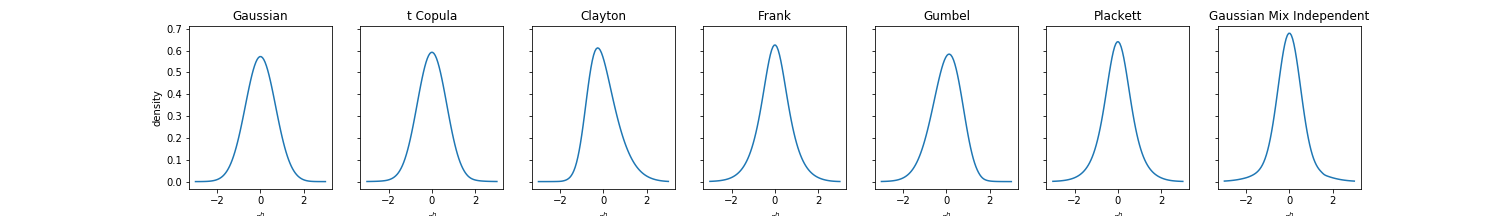
\includegraphics[width=\textwidth]{_pics/density illustration1.png}
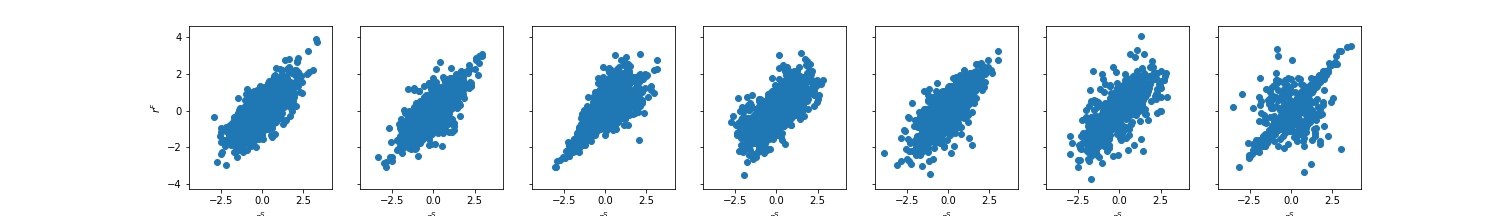
\includegraphics[width=\textwidth]{_pics/density illustration2.png}
  \caption{Upper Panel: Density of $Z= X - hY$ of different copulae with
  $X, Y \sim N(0,1)$,
  $0.75$ Spearman's rho between $X$ and $Y$, and $h=0.5$;
  Lower Panel: Scatter plot of samples from copulae.
  This illustration shows how dependence structure modelled by different copulae affects the density of the linear combination
  of margins.
  Notice that the $Z$ modelled by the asymmetric copulae, namely the Clayton and Gumbel copulae, are skewed to right
  and left respectively. \href{http://www.quantlet.com/}{
\includegraphics[width=15pt]{_pics/qletlogo_tr.png}}}
\label{fig:density illustration}
\end{figure}


The optimality of our hedge is determined by various risk measures,
they include variance, expected shortfall (ES), value-at-risk (VaR),
and spectral risk measures (SRM). \natp{\em [Careful with wording! The
  hedge is not optimal. The optimal hedge ratio that minimises a risk measure is chosen.]}
In particular, the SRM proposed by \citet{Acerbi2002} accounts for investors' utility (i.e. risk preference).
SRM is a weighted average of the quantities of a loss distribution, the weights of which depend on the investor's risk-aversion.
In other words, the risk estimation is directly related to the user's utility function.
Popular examples are the exponential SRM and power SRM introduced by
\citet{dowd2008spectral}. \medskip

%Even though they reveal that SRM have some properties which cause problems when applying to practical risk management,
%they show that exponential utility function might be plausible in some circumstances under weak conditions \citealp{buhlmann1980economic}.

%However, it still causes some problems to capture the behaviors of investors when the value of absolute risk aversion (ARA) parameter beyond a threshold \citealp{markowitz2014mean}.
%If the relative risk aversion coefficients (RRA) are less than 1, \citet{dowd2008spectral} address that the weighting of lower risk-averse is higher than the higher risk-averse as the loss of portfolio increases.
%On the other hand, the power SRM proposed by \citet{dowd2008spectral} when the relative risk aversion coefficients (RRA) are larger than 1, has also proper features to give a higher weight as loss increase.
%Note that the selection of the utility function and the value of risk aversion parameter would be the matters of solving specific financial problem.
%By contrast, the estimation of the VaR and the ES are conditional on the confidence level which is not easy to determine.
%Since SRM is capable of reflecting the investor's attitude toward risk and has been applied to various fields of financial decision making, this paper apply to the determination of the optimal hedge ratio.
%It is important for the hedger who should choose a proper value for the hedge ratio in order to minimize the risk of portfolio.\\
%
%A joint distribution of spot and futures has been specified in terms of a copula function to embody the tail behaviors of the spot and the futures \citealp{barbi2014copula}.
%Copulae enable us to build the flexible multivariate distributions of dependence structure.
%This paper conducts four types of copulae (Gaussian, t, Frank, Clayton, and Normal Inverse Gaussian) to derive the copula representation of quantities to reach copula-based SRM of the hedged portfolio.
%It should be noted that the Clayton copula can be also used to construct the joint distribution with right tail dependence. Frank copula is symmetric and appropriate for data that exhibit weak or no tail dependence. Normal Inverse Gaussian (NIG) copula is a flexible system of joint distribution that includes fat-tailed and skewed distributions. However, there is still no evidence yet for selecting an exclusive copula in applications of hedging.\\
%
%An optimal hedge ratio represents the investor's subjective marginal rate of substitution between risk and return. \citet{cecchetti1988estimation} found that the optimal hedge ratios increases when an investor with a greater risk aversion by maximizing the expected value of the logarithm of wealth.
%It is understandable if a investor's attitude is more risk-averse, they will increase the position of futures contracts to hedging the uncertain risk which they may take in the future.
%On the contrary, \citet{brandtner2015decision} address that the theoretical result predictions for the subset of exponential and power SRMs are not reasonable but may be counter-intuitive if the corresponding parameter of risk aversion is large enough.
%Different from \citet{brandtner2015decision}, we consider the joint distribution of financial assets to choose the optimal hedge ratio by minimizing SRM.
%However, the empirical result shows the direction of optimal hedge ratio is increasing as the parameters represents the investors' attitude increases. \\

%This paper has two main contributions to the existing literature. First, we reveal the quantiles of loss function built by different copulae. Second, by minimizing exponential SRM (ESRM) to determine the optimal hedge ratio, we give a guidance on the choice of risk aversion function to assist the risk manager in choosing an optimal risk aversion function for a portfolio. To our knowledge, these have received no attention so far in the published literatures.\\

TODO: "What do we find" \medskip

The remainder
of the article is organized as follows. Section 2 methodology. Section 3 data, and Section 4 empirical result. Section 5 concludes.\medskip

All calculations in this work can be reproduced.
The codes are available on \href{http://www.quantlet.com/}{www.quantlet.com}.
%%%%%%%%%%%%%%%%%%%%%%%%%%%%%%%%%%%%%%%%%%%%%%%%%%%%%%%%%%%%%%%%%%%%%%%%%%%%%%

\section{Optimal hedge ratio $h^*$}
\label{sec:optimal-hedge-ratio}

\natp{\em [Try to avoid mathematical notation in section
  headings. Also, avoid mathematical notation at the beginning of a
  sentence. Formulate {\bf carefully}! For example: ``The hedged
  portfolio is $Z=X-hY$.'' is not precise. First, $X$ and $Y$ have not
  been introduced. Second $Z$ refers to the portfolio return. Third,
  $Z$ refers to {\em any\/} portfolio. It is not explained why this
  would be a hedge. Below is a suggestion, now go through the text and
  formulate carefully what you want to say. This takes time...]}

\natp{Let $r_S$ and $r_F$ be the returns of the spot and futures price
  of an asset. The hedged position is a portfolio with return $r_h =
  r_S - h r_F$, where the amount $h$ of futures to short is chosen to
  minimise the risk of the exposure in the spot. (was: 
Consider the problem of an optimal
hedge ratios by risk measures and dependence
structures.
The hedged portfolio is $Z = X - h Y$.
It involves returns of two assets $X$ and $Y$.
This is the situation where we long one unit of asset $X$ and short $h$ unit of asset $Y$.
$h$ is called the hedge ratio.)}
We denote the risk measure of the returns of the hedged portfolio $Z$ as $\rho(Z)$. \medskip
\natp{\em [Again: Introduce $\rho$ as being a risk measure on financial
  positions, i.e., a mapping from a financial position to a real
  number (see e.g.\ McNeil, Chapter 6 or the book by F\"ollmer Schied).]} 

The optimal hedge ratio is $h^\ast = \argmin_h \rho(Z)$, that is the best ratio that can minimize the risk of a hedged portfolio measured in terms of $\rho$ . \medskip

\natp{\em [Introduce the definition of copulas here. Also, this is a
  good place to motivate the separate modelling of dependence and
  margins. First, explain that the ability to hedge is driven by the
  dependence in $r_S$ and $r_F$. And so on. ]}
The distribution function of $Z$ can be expressed in terms of the
copula and the marginal distributions as Proposition \ref{prop:dfrh}
result shows (this is a corrected version of Corollary 2.1 of
\citep{barbi2014copula}). For practical applications, it is numerically
faster and more stable to use additional information about the
specific copula and marginal distributions. \natp{\em [What do you
  mean by additional information? Fast than what?]} We therefore derive
semi-analytic formulae for a number of special cases, such as the
Gaussian-, Student $t$-, normal inverse Gaussian (NIG) and Archimedean
copulas in Section \ref{subsec:copulae}.

\natp{\em [What is the purpose of the parameters $w$ and $\lambda$
  below? Leave them out here and use them where they are needed.]}

\begin{proposition}
  \label{prop:dfrh}
  Let $X$ and $Y$ be two real-valued \natp{continuous} random
  variables on \natp{a (was: the same)}
  probability space $(\Omega, \mathcal A, \p)$ with \natp{(delete: corresponding)}
  absolutely continuous copula $C_{X, Y}$ and
  \natp{(delete: continuous)} marginal distribution functions $F_{X}$
  and $F_{Y}$. Then, the distribution function of of $Z$ is given by 
  \begin{equation}
    \label{eq:3}
    F_{Z}(z) = 1- \int^1_0 D_1 C_{X, Y}
    \left[ u, F_{Y} \left\{ \frac{F^{(-1)}_{X}(u)-z}{h} \right\}
    \right]\, d u.
  \end{equation}
\end{proposition}
Here, $F^{(-1)}$ denotes the inverse of $F$, i.e., the quantile
function. \natp{\em [Spell out inverse function, with $\inf$.]}

Here $D_1 C(u,v)=\displaystyle \frac{\partial}{\partial u} C(u,v)$,
which is easily shown to fulfil, see e.g.\ Equation (5.15) of
\citep{McNeil2005}:
\begin{equation}
  \label{eq:1}
  D_1 C_{X,Y}(F_X(x), F_Y(y)) = \p(Y\leq y|X=x).
\end{equation}
\begin{proof}
  \natp{\em [Use blackboard E as expectation operator, i.e., $\E$.]}
  Using the identity (\ref{eq:1}) gives
  \begin{align*}
    F_{Z}(z) &= \p(X - h Y\leq z) %
                 = \mbox{\sf E}\left\{\p\left(Y\geq \frac{X-z}{h}\Big|
                 X\right)\right\}\\[10pt]
               &= 1-\mbox{\sf E}\left\{\p\left(Y\leq \frac{X-z}{h}\Big|
                 X\right)\right\}% \\[10pt]
               = 1- \int_0^1 D_1 C_{X, Y}\left[u,
                 F_{Y}\left\{\frac{F^{(-1)}_{X}(u) -
                 z}{h}\right\}\right]\, d u.
  \end{align*}
  \end{proof}


In addition to~\cite{barbi2014copula} we propose a more handy
expression for the density of $Z$. \natp{\em [Is this used later? If
  not, thenn possibly remove. If it stays, then make this a
  corollary. Fix punctuation below. Also, please double-check the
  ``+'' signs in the second equation.]}

\begin{prop} Given the formulation of the above portfolio, the density of $Z$ can be written as
  \begin{align}
  f_{Z}(z) &= \left|\frac{1}{h}\right|\int_0^1 c_{X, Y} \left[
  F_{Y}\left\{\frac{F^{(-1)}_{X}(u)-z}{h}\right\}, u
  \right]
   \cdot
  f_{Y}
  \left\{\frac{F^{(-1)}_{X}(u)-z}{h}\right\} du \label{eq:density1}
  \end{align}, or
    \begin{align}
      f_{Z}(z)
      = \int_0^1 c_{X, Y} \left[
      F_{X}\left\{z + h F^{(-1)}_{Y}(u)\right\}, u
      \right]
       \cdot
      f_{X}
      \left\{
      z+ hF^{(-1)}_{Y}(u).
      \right\} du\label{eq:density2}
  \end{align}
  \end{prop}
The two expression are equivalent, one can use any of them to get the
density of $Z$. \natp{\em [Reformuate... why ``get the density''? They
  {\bf are} the density, no?]}
Notice that the density of $Z$ in the above proposition is readily accessible as long as we have
the copula density and the marginal densities.
The proof and a generic expression can be found in the
appendix. \medskip

\natp{\em [Portfolios. Not aware that portfolio is a Latin word.]}

In this work, we consider two portfolios: $R^h = R^{\text{BTC}} - h R^{\text{future}}$ and $R^h = R^{\text{BTC}} - h R^{\text{CRIX}}$.

\natp{\em [For now, stick to $r_S$ and $r_F$. This is still the
  general part, so no need to mention Bitcoin, CRIX, etc. here. Also,
  wasn't the idea to hedge CRIX with the future? I don't see why CRIX
  would be used to hedge Bitcoin when futures are readily
  available. Entering into futures contracts requires no notional,
  which makes them ideal for hedging.]}

%OLD
%\section{Methodology}\label{sec:methodology}
%Following \citet{barbi2014copula}, we consider the problem of optimal
%hedge ratios by extending the commonly known minimum variance hedge
%ratio to more general risk measures and dependence
%structures.\medskip
%
%Hedge portfolio: $R_t^h = R_t^S - h R_t^F$, involving returns of spot
%and future contract and where $h$ is the hedge ratio.\medskip
%
%The optimal hedge ratio is
%\begin{align}
%    h^\ast = \argmin_h \rho_\phi(s,h),
%    \end{align}
%for given
%confidence level $1-s$ (if applicable, e.g.\ in the case of VaR, ES),
%where $\rho_\phi$ is a spectral risk measure with weighting function
%$\phi$ (see below).
%In other words, our task is to search for the optimal $h$ which can minimize a particular risk measure.
%We call the risk measure being used in search process of $h^\ast$ risk reduction objective.
%This naming is to differentiate the risk objective and risk outcome.
%One can see from result section that the $h^\ast$ which minimize a particular risk measure in training does not
%necessarily minimize the risk measure in testing data.
%For example in table \ref{OOSRHVaR99}, the best performing risk reduction objective to reduce out-of-sample Value-at-Risk 99\% is
%exponential risk measure $k=10$. \medskip
%
%The distribution function of $Z$ can be expressed in terms of the
%copula and the marginal distributions as Proposition \ref{prop:dfrh}
%result shows (this is a corrected version of Corollary 2.1 of
%\citep{barbi2014copula}). For practical applications, it is numerically
%faster and more stable to use additional information about the
%specific copula and marginal distributions. We therefore derive
%semi-analytic formulas for a number of special cases, such as the
%Gaussian-, Student $t$-, normal inverse Gaussian (NIG) and Archimedean
%copulas in Section \ref{sec:dependence}.
%
%\begin{proposition}
%  \label{prop:dfrh}
%  Let $X$ and $Y$ be two real-valued random variables on the same
%  probability space $(\Omega, \mathcal A, p)$ with corresponding
%  absolutely continuous copula $C_{X, Y}(w,\lambda)$ and
%  continuous marginals $F_{X}$ and $F_{Y}$. Then, the distribution
%  of of $Z$ is given by
%  \begin{equation}
%    \label{eq:3}
%    F_{Z}(x) = 1- \int^1_0 D_1 C_{X, Y}
%    \left( u, F_{Y} \left( \frac{F^{(-1)}_{X}(u)-x}{h} \right)
%    \right)\, d u.
%  \end{equation}
%\end{proposition}\medskip
%Here $D_1 C(u,v)=\displaystyle \frac{\partial}{\partial u} C(u,v)$,
%which is easily shown to fulfil, see e.g.\ Equation (5.15) of
%\citep{McNeil2005}:\footnote{%
%  Let $F_X(x)=u$, $F_Y(y)=v$. Then, formally,
%  \begin{align*}
%    \frac{\partial}{\partial F_X(x)} C(F_X(x), F_Y(y)) %
%    &= \frac{\partial}{\partial F_X(x)} \p(U\leq F_X(x),
%      V\leq F_Y(y)) %
%      = \p(U\in d F_X(x), V\leq F_Y(y))\\ %
%    &= \p(V\leq F_Y(y)| U = F_X(x))\cdot \p(U \in d
%      F_X(x)) %
%      = \p(Y\leq y|X=x)\cdot \p(U\in d u)\\ %
%    &= \p(Y\leq y|X=x).
%  \end{align*}}
%\begin{equation}
%  \label{eq:1}
%  D_1 C_{X,Y}(F_X(x), F_Y(y)) = \p(Y\leq y|X=x).
%\end{equation}
%\begin{proof}
%  Using the identity (\ref{eq:1}) gives
%  \begin{align*}
%    F_{Z}(x) &= \p(R^s - h Y\leq x) %
%                 = \E\left[\p\left(Y\geq \frac{X-x}{h}\Big|
%                 X\right)\right]\\[10pt]
%               &= 1-\E\left[\p\left(Y\leq \frac{X-x}{h}\Big|
%                 X\right)\right]% \\[10pt]
%               = 1- \int_0^1 D_1 C_{X, Y}\left(u,
%                 F_{Y}\left(\frac{F^{(-1)}_{X}(u) -
%                 x}{h}\right)\right)\, d u.
%  \end{align*}
%\end{proof}\medskip
%
%In addition to \cite{barbi2014copula} we propose an expression for the density of $Z$
%
%\begin{proposition} With the same setting of the above proposition, the density of $Z$ can be written as
%  \begin{align}
%  f_{Z}(y) &= \left|\frac{1}{h}\right|\int_0^1 c_{X, Y} \left[u,
%  F_{Y}\left\{\frac{F^{(-1)}_{X}(u)-y}{h}\right\}
%  \right]
%   \cdot
%  f_{Y}
%  \left\{\frac{F^{(-1)}_{X}(u)-y}{h}\right\} du \label{eq:density1}
%  \end{align}, or
%    \begin{align}
%      f_{Z}(y)
%      = \int_0^1 c_{X, Y} \left[u,
%      F_{X}\left\{y + h F^{(-1)}_{Y}(u)\right\}
%      \right]
%       \cdot
%      f_{X}
%      \left\{
%      y+ hF^{(-1)}_{Y}(u)
%      \right\} du.\label{eq:density2}
%  \end{align}
%  \end{proposition}

% ----------------
% --- Describe the methodology of finding the optimal h ---
% ----------------

\subsection{Spectral Risk Measures}\label{subsec:spectral-risk-measures}
Following \citet{dowd2008spectral}, the spectral risk measures (SRM) of a hedged portfolio return $R^h$ has a form

\begin{align}
	\rho_\phi(R^h) = - \int_0^1 \phi(p) F_{R^h}^{-1}(p)\dd p,
	\end{align}

where $p$ is the loss quantile and $\phi(p)$ is a user-defined weighting function defined over $[0,1]$. \medskip

Spectral risk measures can also be written as
\begin{align}
	\rho_\phi(R^h) = - \int_\mathbb{R} x f_{R^h}(x) \phi\{F_{R^h}(x)\} \dd x.
	\end{align}

Value-at-Risk (VaR) and Expected Shortfall (ES) fall in to the class of SRM.
VaR at the $\alpha$-confidence level is

\begin{align}
	\text{VaR}_\alpha = - F_{R^h}^{-1}(1-\alpha)
	\end{align};
ES at the $\alpha$-confidence level is
\begin{align}
	\text{ES}_\alpha = \frac{1}{1-\alpha}\int_{-\infty}^{\alpha} F_{R^h}^{-1}(p) \dd p
	\end{align}.
The VaR's $\phi(p)$ gives all its weight on the $\alpha$ quantile of $R^h$ and zero elsewhere, i.e. the weighting function is a Dirac delta function.
The ES' $\phi(p)$ gives all tail quantiles the same weight of $\frac{1}{1-\alpha}$ and non-tail quantiles zero weight. \medskip

Spectral risk measures take account of investor's risk aversion by using different $\phi(p)$.
Exponential spectral risk measures (ERM) as a kind of spectral risk measure take a form of the weight function

\begin{align}
	\phi(p) =\frac{k e^{-k(1-p)}}{1-e^{-k}} ,
	\end{align}
where $k$ is the Arrow-Pratt coefficient of absolute risk aversion. \medskip

$k$ has an economic interpretation of being the ratio between the second derivative and first derivative
of investor's utility function on an risky asset

\begin{align}
	k = -\frac{U''(x)}{U'(x)},
	\end{align}
for $x$ in all possible outcomes.
A summary of risk measures being used in portfolio selection probelm can be found in \citet{hardle2008applied}.\medskip

In this hedging study, variance and the risk measures mentioned above serve as a loss function determining the optimality
of $h^\ast$.

\begin{figure}[h]
	\begin{center}
		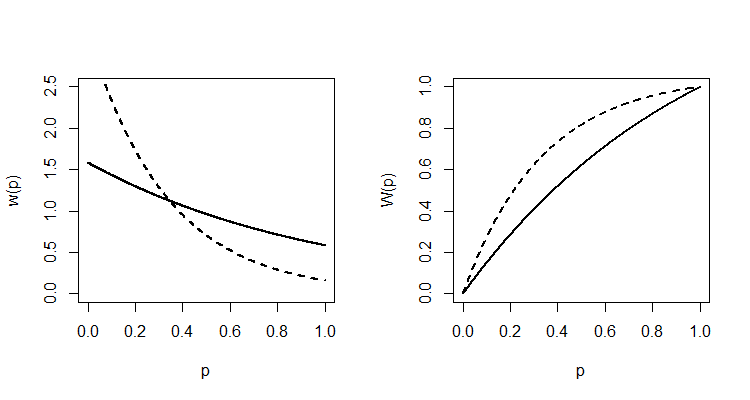
\includegraphics[scale = 0.7]{Figures/Fig1-1.png}\\
		%\vspace*{-10pt}\quantnet \href{https://github.com/mangrou/SRM/blob/master/SRM_QF/SRM_QF.m}{SRM\_QF}
	\end{center}
	\caption{Exponential SRMs for $k=1$ (dashed) and $k=2$ (solid).}\label{Fig1:EPSRM}
\end{figure}

% ----------------
% --- Risk measures' definition and properties ---
% ----------------

\documentclass[square]{article} %
\usepackage{amsfonts,amssymb,amsthm} %
\usepackage[tbtags]{amsmath} %
\usepackage{bm}
\newtheorem{theorem}{Theorem}
\newtheorem{prop}{Proposition}
\newtheorem{eg}{Example}


\begin{document}
    Copula is a function represent the multivariate structure of random variables.
    Frechet-Hoeffding lower bound $\bm{W}(u,v) = \min(u,v)$, Frechet-Hoeffding upper bound $\bm{M}(u,v) = \max(u+v-1,0)$,
    and product copula $\bm{\Pi}=uv$ are three important special instants of copulas.
    They describe the perfect counter-dependence, perfect dependence, and independence of two random variables, respectively.
    The inequality $\bm{W}(u,v) \leq \bm{C}(u,v) \leq \bm{M}(u,v)$ holds for every copula $\bm{C}$ ad every $(u,v) \in \mathbb{I}^2$ (Nelsen 2.2.5).

    \section{Ellpitical Copulas}\label{sec:ellpitical-copulas}
%    A random vector $X \in \mathbb{R}^d$ is said to have an elliptical distribution if it admits the stochastic representation
%    \begin{align}
%        \bm{X} = \bm{\mu}+ R\bm{A}\bm{U}
%        \end{align}
%where $\bm{\mu} \in \mathbb{R}^d$, $R$ is a positive random variable independent of $\bm{U}$,
%    $\bm{U}$ is a random vector uniform on the unit sphere in $\mathbb{R}^d$,
%    and $\bm{A}$ is a fixed $d \times d$ matrix such that $\bm{\Sigma} = \bm{A} \bm{A}^\intercal$ is non-singular.
%
%    The density function of an elliptical distribution is given by
%    \begin{align}
%        f(\bm{x}) = |\bm{\Sigma}|^{-\frac{1}{2}} g\{(\bm{x}-\bm{\mu})^\intercal \bm{\Sigma}^{-1}(\bm{x}-\bm{\mu})\}
%        \end{align}
%    for some function $g:\mathbb{R} \rightarrow \mathbb{R}^+$, the density generator.
%    The function g uniquely determine the distriution of $R$ (ref).
%
%    For multivariate Normal distribution, its density generator is
%    \begin{align}
%        g(t)=Ce^{-\frac{t}{2}}
%        \end{align}
%    where $C$ is .
%
%    For multivariate Student-t distribution, its density generator is
%        \begin{align}
%            g(t)=C\left(1+\frac{t}{m}\right)^{-\frac{d+m}{2}}
%        \end{align}
%
%%    An elliptical copula is .
%%    It can also be obtained by method of inversion (see)
%    If $H$ is a $d$-variate elliptical distribution, the corresponding elliptical copula is
%    \begin{align}
%        \bm{C}(\bm{u}) = H(F_{X_1}^{-1}(u_1),\dots, F_{X_d}^{-1}(u_d)).
%        \end{align}

    Elliptical copulas are copulas f elliptical distributions.
    Gaussian copula is the copula associated with multivariate normal distribution.
    The Gaussian copula (B1 in Joe) has a form
        \begin{align}
            \bm{C}(u,v) &= \Phi_{2, \rho}\{\Phi^{-1}(u), \Phi^{-1}(v)\} \\
                        &= \int_{-\infty}^{\Phi^{-1}(u)}
                           \int_{-\infty}^{\Phi^{-1}(v)}
                           \frac{1}{2\pi\sqrt{1-\rho^2}}
                           \exp{\left(
                           \frac{s^2-2\rho st+t^2}{2(1-\rho^2)}
                           \right)} ds dt
            \end{align}
    where $\Phi_{2, \rho}$ is the cdf of bivariate Normal distribution with zero mean, unit variance, and correlation $\rho$,
    and $\Phi^{-1}$ is quantile function univariate standard normal distribution.
    The copula density of Gaussian copula can be written as
    \begin{align}
        \bm{c}_\rho(u,v) &= \frac{\phi_{2,\rho}\{\Phi^{-1}(u), \Phi^{-1}(v)\}}
                            {\phi\{\Phi^{-1}(u)\} \cdot \phi\{\Phi^{-1}(v)\}}\\
                    &= \frac{1}{2\pi\sqrt{1-\rho^2}}\exp\left(
                       -\frac{u^2 - 2\rho uv + v^2}{2(1-\rho^2)}
                       \right) ,
        \end{align}
    where $\phi_{2,\rho}(\cdot)$ is the density of bivariate Normal distribution with zero mean,
    unit variance,
    and correlation $\rho$,
    and, $\phi(\cdot)$ the density of standard normal distribution.

    The Kendall's $\tau_K$ and Spearman's $\rho_S$ of a bivariate Gaussian Copula are
        \begin{align}
            \tau_K(\rho) = \frac{2}{\pi}\arcsin\rho
            \end{align}
        \begin{align}
            \rho_S(\rho) = \frac{6}{\pi}\arcsin\frac{\rho}{2}
            \end{align}

    t copula is associated with multivariate t distribution.
    The t Copula takes a form
    \begin{align}
            \bm{C}(u,v) &= \bm{T}_{2, \rho, \nu}\{T^{-1}_\nu(u), T^{-1}_\nu(v)\} \\
                &= \int_{-\infty}^{T^{-1}_\nu(u)}
                   \int_{-\infty}^{T^{-1}_\nu(v)}
                \frac{\Gamma\left(\frac{\nu+2}{2}\right)}
                {\Gamma\left(\frac{\nu}{2}\right)\pi\nu\sqrt{1-\rho^2}}\\
               & \left(
            1+\frac{s^2-2st\rho+t^2}{\nu}
            \right)^{-\frac{\nu+2}{2}} ds dt,
        \end{align}
    where $\bm{T}_{2, \rho, \nu}(\cdot, \cdot)$ denotes the cdf of bivariate t distribution with scale parameter $\rho$ and degree of free $\nu$,
    $T^{-1}_\nu(\cdot)$ is the quantile function of a standard t distribution with degree of freedom $\rho$.

    The copula density is
    \begin{align}
        \bm{c}(u,v) &= \frac{\bm{t}_{2, \rho, \nu}\{T^{-1}_\nu(u), T^{-1}_\nu(v)\}}
        {t_\nu\{T^{-1}_\nu(u)\}\cdot t_\nu\{T^{-1}_\nu(v)\}},
        \end{align}
    where $\bm{t}_{2,\rho, \nu}$ is the density of bivariate t distribution,
    and $t_\nu$ the density of standard t distribution.

    Like all the other elliptical copula, t copula's Kendall's $\tau$ is same to that of Gaussian copula (Demarta and reference therein).

    \section{Archimedean Copula}\label{sec:archimedean-copula}
    Archimedean copula forms a large class of copulas with many convenient features.

    In general, Archimedean copula takes a form
    \begin{align}
        \bm{C}(u,v)= \psi^{-1}\{\psi(u), \psi(v)\},
        \end{align}
    where $\psi:[0,1] \rightarrow [0,\infty)$ is a continuous, strictly decreasing and convex function such that
    $\psi(1)=0$ for any permissible dependence parameter $\theta$. $\psi$ is also called generator.
    $\psi^{-1}$ is the inverse the generator.

    This section will briefly introduce this class of copula,
    we refer readers to Nelsen and Joe for Detail of this class of copula.

    Frank copula (B3 in Joe) is a radial symmetric copula and does not have any tail dependence.
    It takes the form
    \begin{align}
        \bm{C}_{\theta}(u,v) &= \frac{1}{\log(\theta)}
        \log \left\{
        1 + \frac{(\theta^u-1)(\theta^v-1)}{\theta-1}
        \right\}
        \end{align}
    where $\theta \in [0, \infty]$ is the dependency parameter.
    $\bm{C}_1 = \bm{M}$, $\bm{C}_1 = \bm{\Pi}$, and $\bm{C}_\infty = \bm{W}$.

    The Copula density
    \begin{align}
        \bm{c}_{\theta}(u,v) &= \frac{(\theta-1)\theta^{u+v}\log(\theta)}
        {\theta^{u+v}-\theta^u-\theta^v+\theta}
        \end{align}

    Frank copula has Kendall's $\tau$ and Spearman's $\rho$ as follow:
    \begin{align}
        \tau_K(\theta) = 1-4\frac{D_1\{-\log(\theta)\}}{\log(\theta)},
        \end{align}
and
    \begin{align}
        \rho_S(\theta) = 1-12\frac{D_2\{-\log(\theta)\} - D_1\{\log(\theta)\}}{\log(\theta)},
        \end{align}
    where $D_1$ and $D_2$ are the Debye function of order 1 and 2.
    Debye function is $D_n = \frac{n}{x^n}\int_0^x\frac{t^n}{e^t-1}dt$.

    Gumbel copula (B6 in Joe) has upper tail dependence with the dependence parameter
    $\lambda^U = 2-2^{\frac{1}{\theta}}$ and displays no lower tail dependence.
    \begin{align}
        \bm{C}_{\theta}(u,v) &= \exp{-\{
        (-\log(u))^\theta +(-\log(v))^\theta
        \}^{\frac{1}{\theta}}},
        \end{align}
    where $\theta \in [1,\infty)$ is the dependence parameter.
    While Gumbel copula cannot model perfect counter dependence (ref), $\bm{C}_{1} = \bm{\Pi}$ models the independence,
    and $\lim\limits_{\theta \to \infty} \bm{C}_\theta = \bm{W}$ models the perfect dependence.

    The copula density takes the form
    \begin{align}
            f
        \end{align}

      \begin{align}
        \tau_K(\theta) =\frac{\theta-1}{\theta}
        \end{align}

    Clayton copula, opposite to Gumbel copula,
    generates lower tail dependence in a form $\lambda^L = 2^{-\frac{1}{\theta}}$,
    but generates no upper tail dependence.
    Clayton copula takes a form
    \begin{align}
        \bm{C}_{\theta}(u,v) &= \left[
        \max\{u^{-\theta}+v^{-\theta}-1,0\}\right]^{-\frac{1}{\theta}},
        \end{align}
    where $\theta \in (-\infty, \infty)$ is the dependency parameter.
    $\lim\limits_{\theta \to -\infty} \bm{C}_\theta = \bm{M}$, $\bm{C}_0 = \bm{\Pi}$, and $\lim\limits_{\theta \to \infty} \bm{C}_\theta = \bm{W}$.

    Its Kendall's $\tau$ is
    \begin{align}
        \tau_K(\theta) =\frac{\theta}{\theta+2}.
        \end{align}

    Plackett copula has an expression
    \begin{align}
        \bm{C}_{\theta}(u,v) &= \frac{1+(\theta-1)(u+v)}{2(\theta-1)}
                             - \frac{\sqrt{\{
        1+(\theta-1)(u+v)\}^2 - 4uv\theta(\theta-1)}}{2(\theta-1)}
        \end{align}
    \begin{align}
        \rho_S(\theta) = \frac{\theta+1}{\theta-1} - \frac{2\theta \log \theta}{(\theta-1)^2}
        \end{align}

    We include Placket copula in our analysis as it possesses a special property,
    the cross-product ratio is equal to the dependence parameter
    \begin{align}
        &\phantom{=} \frac{\mathbb{P}(U \leq u, V \leq v) \cdot \mathbb{P}(U > u, V > v)}
        {\mathbb{P}(U \leq u, V > v) \cdot \mathbb{P}(U > u, V \leq v)}\\
        &= \frac{C_\theta(u,v)\{1-u-v+C_\theta(u,v)\}}{\{u-C_\theta(u,v)\}\{v-C_\theta(u,v)}\\
        &= \theta.
        \end{align}
    That is, the dependence parameter is equal to the ratio between number of concordence pairs and number of discordence pairs of a bivariate random variable.
    \section{Mixture Copula}\label{sec:mixture-copula}
    Mixture copula is a linear combination of copulas.
    It allows us to model the dependence structure in a more flexible manner.

    For a 2-dimensional random variable $\bm{X}=(X_1,X_2)^\intercal$,
    its distribution can be written as linear combination $K$ copulas
    \begin{align}
        \mathbb{P}(X_1 \leq x_1, X_2 \leq x_2) = \sum_{k=1}^K p^k \cdot \bm{C}^{(k)}\{F^{(k)}_{X_1}(x_1;\bm{\gamma}^{(k)}_1),
        F^{(k)}_{X_2}(x_2;\bm{\gamma}^{(k)}_2); \bm{\theta^{(k)}}\}
        \end{align}
    where $p^{(k)} \in [0,1]$ is the weight of each component,
    $\bm{\gamma}^{(k)}$ is the parameter of the marginal distribution in the $k^\text{th}$ component,
    and $\bm{\theta^{(k)}}$ is the dependence parameter of the $k^\text{th}$ component.
    We also restrict the weight so that $\sum_{k=1}^K p^{(k)}=1$.
    Analysis of mixture copula with higher dimension can be found in Vrac et. al. (2011).

    We deploy a simplified version of the above representation by assuming the maringals of $\bm{X}$ are not mixture.
    By Sklar's theorem we write
    \begin{align}
        \bm{C}(u,v)= \sum_{k=1}^K p^{(k)} \cdot \bm{C}^{(k)}\{F^{-1}_{X_1}(u),
        F^{-1}_{X_2}(v); \bm{\theta^{(k)}}\}.
        \end{align}

    The copula density is again a linear combination of copula density
    \begin{align}
        \bm{c}(u,v)= \sum_{k=1}^K p^{(k)} \cdot \bm{c}^{(k)}\{F^{-1}_{X_1}(u),
        F^{-1}_{X_2}(v); \bm{\theta^{(k)}}\}.
        \end{align}

    While Kendall's $\tau$ of mixture copula is not known in close form,
    the Spearman's $\rho$ is

    \begin{prop}
        Let $\rho_S^{(k)}$ be the Spearman's $\rho$ of the $k^\text{th}$ component and $\sum_{k=1}^K p^{(k)}=1$ holds,
        the Spearman's $\rho$ of a mixture copula is
        \begin{align}
            \rho_S = \sum_{k=1}^K p^{(k)} \cdot \rho_S^{(k)}
            \end{align}
        \end{prop}

    \begin{proof}
        Spearman's $\rho$ is defined as (Nelsen)
        \begin{align}
            \rho_S = 12 \int_{\mathbb{I}^2} \bm{C}(s,t) ds dt - 3.
            \end{align}
        Rewrite the mixture copula into sumation of components
           \begin{align}
            \rho_S = 12 \int_{\mathbb{I}^2} \sum_{k=1}^K p^{(k)} \cdot \bm{C}^{(k)}(s,t) ds dt - 3.
            \end{align}
        \end{proof}
    \begin{eg}
        Frechet class can be seen as an example of mixture copula.
        It is a convex combinations of $\bm{W}$, $\bm{\Pi}$, and $\bm{M}$ (Nelsen)
        \begin{align}
            \bm{C}_{\alpha, \beta}(u,v)
            = \alpha \bm{M}(u,v) +
            (1-\alpha-\beta)\bm{\Pi}(u,v)
            +\beta \bm{W}(u,v),
            \end{align}
        where $\alpha$ and $\beta$ are the dependence parameters, with $\alpha, \beta \geq 0$ and
        $\alpha+\beta \leq 1$.
        Its Kendall's $\tau$ and Spearman's $\rho$ are
        \begin{align}
            \tau_K(\alpha, \beta) = \frac{(\alpha - \beta)(\alpha+\beta+2)}{3}
            \end{align}
        , and
        \begin{align}
            \rho_S(\alpha, \beta) = \alpha - \beta
            \end{align}
        \end{eg}
    Example 2 Gumbel-Clayton mixture
    Example 3 Hu 2006.

    We use a mixture of Gaussian and independent copula in our analysis.
    We write the copula
    \begin{align}
        \bm{C}(u,v) = p\cdot \bm{C}^\text{Gaussian}(u,v) + (1-p)(uv).
        \end{align}
    The corresponding copula density is
    \begin{align}
        \bm{c}(u,v) = p\cdot \bm{c}^\text{Gaussian}(u,v) + (1-p).
        \end{align}

    This mixture allows us to model how much "random noise" appear in the dependency structure.
    In this hedging exercise, the structure of the "random noise" is not of our concern nor we can
    hedge the noise by a two-asset portfolio.
    However, the proportion of the "random noise" does affect the distribution of $r^h$ (see figure),
    so as the optimal hedging ratio $h$ (see figure).
    One can consider the mixture copula as a handful tool for stress testing.
    Similar to this Gaussian mix Independent copula,
    t copula is also a two parameter copula allow us to model the noise,
    but its interpretation of parameters is not as intuitive as that of a mixture.
    The mixing variable $p$ is the proportion of a manageable (hedgable?) Gaussian copula,
    while the remaining proportion $1-p$ cannot be managed.
    \end{document}
% ----------------
% --- Copulae's definition and properties ---
% ----------------

%! Author = francis
%! Date = 30.10.20


\subsection{Simulated Method of Moments}\label{subsec:simulated-method-of-moments}
This method is suggested by Oh and Patton (2013).
In this setting, rank correlation e.g. Spearman's $\rho$ or Kendall's $\tau$,
and quantile dependence measures at different levels $\lambda_q$
are calibrated against their empirical counterparts.\medskip

Spearman's rho, Kendall's tau, and quantile dependence of a pair $(X,Y)$
with copula $C$ are defined as
\begin{align}
  \rho_S &= 12 \int\int_{I^2} C_{\bm{\theta}}(u,v)\, \dd u\, \dd v-3\label{eq:rho_S}\\
  \tau_K &= 4\mathbb{E}[C_{\bm{\theta}}\{F_X(x), F_Y(y)\}]-1,\\
  \lambda_q &=
  \begin{cases}
    \p(F_X(X)\leq q| F_Y(Y)\leq q) = \displaystyle \frac{C_{\bm{\theta}}(q,q)}{q},
    &\text{ if } q\in (0,0.5],\\
    \p(F_X(X)>q|F_Y(Y)>q) =\displaystyle \frac{1-2q+C_{\bm{\theta}}(q,q)} {1-q},
    &\text{ if } q\in (0.5,1).
  \end{cases}
\end{align}\medskip
The empirical counterparts are
\begin{align*}
  \hat\rho_S &= \frac{12}{n} \sum_{k=1}^n \hat F_X(x_k) \hat F_Y(y_k)
               -3,\\
  \hat\tau_K &= \frac{4}{n}\sum_{k=1}^n \hat{C}\{\hat{F}_X(x_i),\hat{F}_X(y_i)\} -1 ,\\
  \hat\lambda_q &=
                  \begin{cases}
                    \displaystyle\frac{1}{n} \sum_{k=1}^n \frac{\1_{\{\hat
                        F_X(x_k)\leq q, \hat F_Y(y_k)\leq q\}}} {q},
                    &\text { if } q\in (0, 0.5],\\
                    \displaystyle \frac{1}{n} \sum_{k=1}^n
                    \frac{\1_{\{\hat F_X(x_k)>q, \hat F_Y(y_k)>q\}}}
                    {1-q}, &\text { if } q\in (0.5,1).
                  \end{cases},
\end{align*}
where $\hat{F}(x) := \frac{1}{n}\sum_{k=1}^n 1_{\{x_i\leq x\}}$ and
$\hat{C}(u,v) := \frac{1}{n}\sum_{k=1}^n 1_{\{u_i\leq u, v_i\leq v\}}$.\medskip

We denote $\tilde{\bm{m}}(\bm{\theta})$ be a $m$-dimensional vector of dependence measures according the the
dependence parameters $\bm{\theta}$,and  $\hat{\bm{m}}$ be the corresponding empirical counterpart.
The difference between dependence measures and their counterpart is denoted by
\begin{align*}
    \bm{g}(\bm{\theta}) = \hat{\bm{m}} - \tilde{\bm{m}}(\bm{\theta}).
\end{align*}\medskip

The SMM estimator is
\begin{align*}
    \hat{\bm{\theta}} = \argmin_{\bm{\theta}\in \bm{\Theta}} \bm{g}(\bm{\theta})^\intercal
    \hat{\bm{W}}
     \bm{g}(\bm{\theta}),
\end{align*}
where $\hat{W}$ is some positive definite weigh matrix.\medskip

In this work, we use $\tilde{\bm{m}}(\bm{\theta}) = (\rho_S, \lambda_{0.05}, \lambda_{0.1},
\lambda_{0.9}, \lambda_{0.95})^\intercal$
for calibration of Bitcoin price and CME Bitcoin future.

\subsection{Maximum Likelihood Estimation}\label{subsec:maximum-likelihood-estimation}
By Sklar's theorem, the joint density of a $d$-dimensional random variable $\bm{X}$ with sample size $n$ can be written as
\begin{align}
    \bm{f}_{\bm{X}}(x_1, ..., x_d) = \bm{c}\{F_{X_1}(x_1), ..., F_{X_d}(x_d)\} \prod_{j=1}^d f_{X_i}(x_i).
    \end{align}
We follow the treatment of MLE documented in section 10.1 of \citet{joe1997multivariate}, namely the inference functions for margins or IFM method.
The log-likelihood $\sum^n_{i=1}f_{\bm{X}}(X_{i,1}, ..., X_{i,d})$ can be decomposed into dependence part and marginal part,
\begin{align}
    L(\bm{\theta}) &= \sum_{i=1}^n \bm{c}\{F_{X_1}(x_{i,1};\bm{\delta}_1), ..., F_{X_d}(x_{i,d}; \bm{\delta}_d);\bm{\gamma}\}
    + \sum_{i=1}^n \sum_{j=1}^d f_{X_j}(x_{i,j};\bm{\delta}_j)
    &= L_C(\bm{\delta}_1, ..., \bm{\delta}_d, \bm{\gamma}) + \sum_{j=1}^d L_j(\bm{\delta}_j)
    \end{align}
where $\bm{\delta}_j$ is the parameter of the $j$-th margin, $\bm{\gamma}$ is the parameter of the parametric copula, and
$\bm{\theta} = (\bm{\delta}_1,..., \bm{\delta}_d, \bm{\gamma})$.

Instead of searching the $\bm{\theta}$ is a high dimensional space, \citet{joe1997multivariate} suggests to
search for $\hat{\bm{\delta}_1},..., \hat{\bm{\delta}_d}$ that maximize $L_1(\bm{\delta}_1), ..., L_d(\bm{\delta}_d)$,
then search for $\hat{\bm{\gamma}}$ that maximize $L_C(\hat{\bm{\delta}_1},..., \hat{\bm{\delta}_d}, \bm{\gamma})$.

That is, under regularity conditions, $(\hat{\bm{\delta}_1},..., \hat{\bm{\delta}_d}, \hat{\bm{\gamma}})$ is the solution of
\begin{align}
    \left( \frac{\partial L_1}{\partial \bm{\delta}_1}, ..., \frac{\partial L_d}{\partial \bm{\delta}_d},
    \frac{\partial L_C}{\partial \bm{\gamma}}\right) = \bm{0}.
    \end{align}

However, the IFM requires making assumption to the distribution of of the margins.
\citet{genest1995semiparametric} suggests to replace the estimation of marginals parameters estimation by non-parameteric estimation.
Given non-parametric estimator $\hat{F}_i$ of the margins $F_i$, the estimator of the dependence parameters $\bm{\gamma}$ is
\begin{align}
    \hat{\bm{\gamma}} = \argmax_{\bm{\gamma}} \sum_{i=1}^n \bm{c}\{ \hat{F}_{X_1}(x_{i,1}), ..., \hat{F}_{X_d}(x_{i,d});\bm{\gamma}\}.
    \end{align}



%With the decomposition, the MLE estimator for a bivariate parametric copula is
%\begin{align}
%    \hat{\bm{\theta}} = \argmax_{\bm{\theta} \in \bm{\Theta}} l(X_1,X_2; \bm{\theta}), \label{eq:EMLE}
%    \end{align}
%where
%\begin{align}
%    l(X_1,X_2; \bm{\theta}) = \sum_{i=1}^n \log c(x_{i,1}, x_{i,2};\bm{\theta}). \label{eq:Likelihood}
%    \end{align}\medskip

%Procedure of maximising equation~\ref{eq:EMLE} as a whole is called exact maximum likelihood method.
%Leveraging the attractive feature of copula that one can model the dependence structure and marginals separately,
%we rewrite~\ref{eq:Likelihood} into canonical expression
%\begin{align}
%    l(X,Y; \bm{\theta}) = \sum_{k=1}^n \log c\{F_X(x_i; \delta_X), F_Y(y_i; \delta_Y); \bm{\gamma}\}
%    + \sum_{k=1}^n \log f_X(x_i; \bm{\delta}_X) + \sum_{k=1}^n \log f_X(y_i; \bm{\delta}_Y),
%    \end{align}
%where the $\bm{\gamma}$ is the dependence parameter in the copula and $\bm{\delta}$ is the parameters in the margins.\medskip
%
%The inference-functions for margins (IFM) approach by Joe is a two step procedure of maximising~\ref{eq:EMLE}.
%The approach calibrate first the $\bm{\delta}$s and then the  $\bm{\gamma}$.\medskip
%
%Similar to the IFM approach, pseudo-maximum likelihood approach by Genest and Rivest (1993) replace the parametric margins by
%empirical estimates, we rewrite \ref{eq:Likelihood} again with
%\begin{align}
%    l(X,Y; \bm{\theta}) = \sum_{k=1}^n \log c(u_i, v_i;\bm{\gamma}),
%    \end{align}
%where $u_i = \hat{F}_X(x_i)$ and $v_i = \hat{F}_Y(y_i)$.

\subsection{Comparison}
Both the simulated method of moments and the maximum likelihood estimation are unbiased and
proven to give good fits.
The problem remain is which procedure is more suitable for hedging.
%Cryptocurrencies are known to be very volatile.
Sample and fitted quantile dependence for Bitcoin and CME future.

%\begin{figure}[th]
%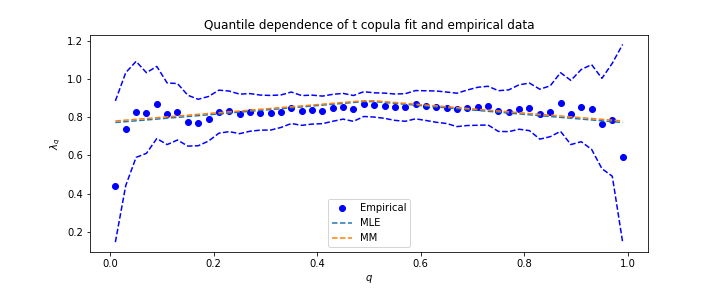
\includegraphics[width=\textwidth]{_pics/t Copula quantile dependence.png}
%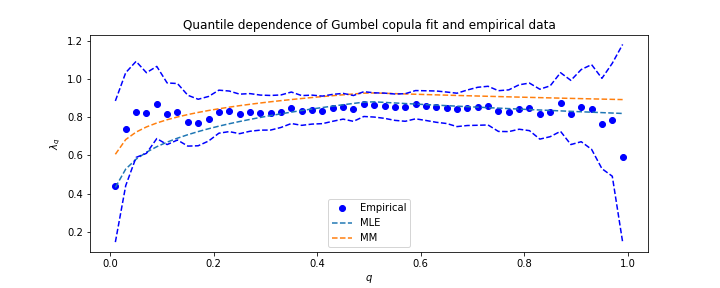
\includegraphics[width=\textwidth]{_pics/Gumbel Copula quantile dependence.png}
%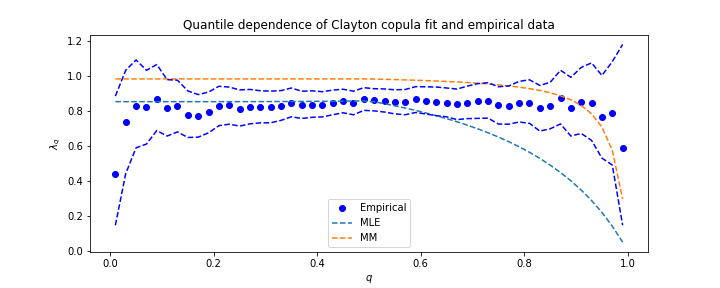
\includegraphics[width=\textwidth]{_pics/Clayton Copula quantile dependence.png}
%  \caption{}
%\label{fig:quantile dependence1}
%\end{figure}


The MM estimation perform just as we decided: match the upper and lower quantile dependence.




%
%
%\subsection{Two-Stage Estimation}\label{subsec:two-stage-estimation}
%~\cite{joe2005asymptotic} study the efficiency of a two-stage estimation procedure of copula estimation.
%The authors also call this method inference function for margins IFM.
%
%\textbf{Pros}
%\begin{enumerate}
%    \item Almost as efficient as MLE methods but easier to be implemented
%    \item Yields an asymptotically Gaussian, unbiased estimate
%\end{enumerate}
%
%\textbf{Cons}
%\begin{enumerate}
%    \item Subject to specification of marginals \cite{kim2007comparison}
%\end{enumerate}
%
%Our data
%\begin{align}
%    \pmb{y} = \begin{bmatrix}
%                  y_{11} & \cdots & y_{1i}\\
%                  \vdots & \ddots & \vdots \\
%                  y_{n1} & \cdots & y_{ni}
%                  \end{bmatrix}
%    \end{align}
%Let $F$ and $f$ be the joint cdf and joint density of $\pmb{y}$ with parameters $\pmb{\delta}$,
%and let $F_i$ and $f_i$ be the marginal cdf and marginal density for the $i^\text{th}$ random variable with parameters $\pmb{\theta}_i$, we have
%\begin{align}
%    f(\pmb{y}; \pmb{\theta}_1, \pmb{\theta}_2,\dots \pmb{\theta}_i, \pmb{\delta}) =
%    c\{F_1(\pmb{y}_1;\pmb{\theta}_1), F_2(\pmb{y}_2; \pmb{\theta}_2), \dots, F_i(\pmb{y}_1;\pmb{\theta}_i); \pmb{\delta}\}
%    \prod^i_{j=1}f_i(\pmb{y}_j;\pmb{\theta}_j)
%    \end{align}
%
%For a sample of size $n$, the log-likelihood of functions of the $i^\text{th}$ univariate margin is
%\begin{align}
%    L_i(\theta_i) = \sum^n_{m=1} \log f_i(y_{mi}; \theta_i),
%    \end{align}
%
%and the log-likelihood function for the joint distribution is
%\begin{align}
%    L(\delta, \theta_1, \theta_2, \dots, \theta_i) = \sum^n_{m=1}\sum^i_{j=1} \log f(y_{mj}; \delta, \theta_1, \theta_2, ..., \theta_i)
%    \end{align}
%
%In most cases, one does not have closed form estimators and numerical techniques are needed.
%Numerical ML estimation difficulty increase when the total number of parameters increases.
%The two-stage estimation is designed to overcome this problem.
%
%The two-stage procedure is
%\begin{enumerate}
%    \item estimate the univariate parameters from separate univariate likelihoods to get $\tilde{\pmb{\theta}_1}, ..., \tilde{\pmb{\theta}_i}$
%    \item maximize $L(\pmb{\delta}, \tilde{\pmb{\theta}_1}, \dots, \tilde{\pmb{\theta}_i})$ over $\pmb{\delta}$ to get $\tilde{\pmb{\delta}}$
%    \end{enumerate}
%
%Under regularity conditions
%\footnote{Regularity conditions include
%1. $\exists \frac{\partial \log f(x;\theta)}{\partial \theta}, \frac{\partial^2 \log f(x;\theta)}{\partial \theta^2}, \frac{\partial^3 \log f(x;\theta)}{\partial \theta^3}$ for all $x$;
%2. $\exists g(x), h(x) and H(x)$ such that for $\theta$ in a neighborhood $N(\theta_0)$ the relations
%$\left|\frac{\partial f(x;\theta)}{\partial theta}\right| \leq g(x)$,
%$\left|\frac{\partial^2 f(x;\theta)}{\partial \theta^2}\right| \leq h(x)$,
%$\left|\frac{\partial^3 f(x;\theta)}{\partial \theta^3}\right| \leq H(x)$ hold for all $x$, and
%$\int g(x) dx < \infty$, $\int h(x) dx < \infty$, $\mathbb{E}_\theta \{H(X)\} < \infty$ for $\theta \in N(\theta_0)$;
%3. For each $\theta \in \Theta$, $0< \mathbb{E}_\theta \left\{
%\left(
%\frac{\partial \log f(X;\theta)}{\partial \theta}
%\right)^2
%\right\}$. For detail see section 4.2.2 of~\cite{serfling2009approximation}}
%, $(\pmb{\tilde{\theta}}_1,\dots \pmb{\tilde{\theta}}_i, \pmb{\tilde{\delta}})$ is the solution of
%\begin{align}
%    (\partial L_1 / \partial \pmb{\theta}^\intercal_1,
%    \dots, \partial L_i / \partial \pmb{\theta}^\intercal_i, \partial L / \partial \pmb{\pmb{\delta}}^\intercal_1) = \pmb{0}
%    \end{align}
%
%For comparison, if we optimize $L$ directly without the two-stage procedure (i.e.~MLE), we solve for
%\begin{align}
%    (\partial L / \partial \pmb{\theta}^\intercal_1,
%    \dots, \partial L / \partial \pmb{\theta}^\intercal_i, \partial L / \partial \pmb{\pmb{\delta}}^\intercal_1) = \pmb{0}
%    \end{align}
%
%We denote the two solutions as
%$\tilde{\pmb{\eta}} = (\pmb{\tilde{\theta}}_1,\dots \pmb{\tilde{\theta}}_i, \pmb{\tilde{\delta}})$ for two-stage procedure;
%$\hat{\pmb{\eta}} =(\pmb{\hat{\theta}}_1,\dots \pmb{\hat{\theta}}_i, \pmb{\hat{\delta}})$ for MLE procedure.
%and compare the asymptotic relative efficiency of $\tilde{\pmb{\eta}}$ and $\hat{\pmb{\eta}}$.
%
%Asymptotics: yet to be done.\\
%~\cite{kim2007comparison} show the estimation of $\pmb{\theta}$ may be seriously affected.
%They compare the two-stage approach and Canonical Maximum Likelihood Method by simulation and
%conclude that Canonical Maximum Likelihood is prefered from a computational statistics and data analysis point of view.
%
%\subsection{Canonical Maximum Likelihood Method}\label{subsec:canonical-maximum-likelihood-method}
%This approach was studied by~\cite{genest1995semiparametric} and~\cite{shih1995inferences}.
%One estimates the margins using empirical CDF
%\begin{align}F_X(x)=\frac{1}{n+1}\sum_{i=1}^n 1(X_i \leq x)\end{align},
%
%we maximize the log-likelihood
%\begin{align}
%    L(\delta) = \sum_{i=1}^n \log [c_\delta \{F_X(X_i), F_Y(Y_i)\}]
%    \end{align}
%
%This procedure does not require specification of marginals.
%
%
%
%
%
%%also by Wang and Ding, 2000; Tsukahara, 2005
%%This is also known as pseudo maximum likelihood (PML) and as canonical maximum likelihood (see Cherubini et al., 2004)
%%
%%Genest and Werker (2002) obtained conditions under which the PMLE is asymptotically efficient.
%%
%%

% ----------------
% --- Estimation of Copula ---
% ----------------

\section{Results}
We illustrate the results in three directions, hedging effectiveness,
ability of hedging extreme negative events in $R^S$, and the stability of $h^*$.

\begin{itemize}
   \item  Hedging Effectiveness
   \begin{itemize}
     \item Kick out Frank for its ineffectiveness; Alternative to a one-parameter symmetric Archimedean copula is Plackett;
     \item Differences among combinations of copula and risk reduction objective are small;
     \item None of the combination can escape from the structural break point (dependence of training is stronger then that of testing). (The bump in 25-26th Sept 2019)
     \item The best performing RRO of a particular risk measure in out-of-sample $R^h$ is not necessarily same, e.g.
      VaR 95\% as RRO (with Gumbel copula) can generate the lowest out-of-sample ES 99\%.
   \end{itemize}
   \item Ability to hedge extreme events in $R^S$
   \begin{itemize}
     \item The extreme events in $R^S$ are well managed by the hedge.
     The magnitudes of loss in $R^h$ is much smaller than that of $R^h$. (Visually seen from the time series of $R^h$)
     \item None of the combination can escape from the structural break point (dependence of training is stronger then that of testing)
   \end{itemize}
   \item Stability of $h^\ast$
   \begin{itemize}
     \item Gumbel gives high $h$ all the time; the extreme events are "hedged" ex-ante.
     \item ES 99\% and VaR 99\% as risk reduction objective are too sensitive to extremes in training data;
     Large changes in $h$ are suggested in response to extremes training data, while the testing data are less extreme;
     \item ERM can be seen as a smoothed risk measure focusing in the lower tail of $R^h$; Less sensitive to rare events; Suggested.
   \end{itemize}
\item \end{itemize}


\subsection{Hedging Effectiveness}\label{subsec:hedging-effectiveness}
The hedging effectiveness(HE) is defined as
\begin{align}
  1- \frac{\rho_\phi(R^h)}{\rho_\phi(R^S)}.
  \end{align}
The hedging effectiveness is the reduction of portfolio risk.
This way of evaluating of hedging performance is proposed by \cite{ederington1979hedging} in the context of, at that time, hedging the newly introduced
organized futures market.
He evaluates the extent of variance reduction by introducing another asset.
We measure the hedging effectiveness also in other risk measure mentioned in section \ref{subsec:spectral-risk-measures},
for example
\begin{align}
  1- \frac{\text{ES}_\alpha(R^h)}{\text{ES}_\alpha(R^S)}.
  \end{align}

The box-plots in figure \ref{fig:OOSHE} show the out-of-sample hedging effectiveness of different copulas under various risk
reduction objectives across testing datasets.
Observe that in most of the copulas perform well in most of the time.
The average HE of copulas and risk reduction objectives is higher than 60\% except for Frank-copula.
However, the HEs vary a lot in different testing data.
In some instances, the HE can be as low as 10\%.
This reflects the highly violate nature of cryptocurrencies:
the optimal hedge ratio in the training data deviates from that of testing data.
There is a large literature about structural break points and time changing dependence, to name a few
\citet{hafner2012dynamic}, \citet{patton2006modelling}, \citet{creal2008general},
\citet{engle2002dynamic}, and \citet{giacomini2009inhomogeneous}.
\citet{manner2012survey} gives a great survey about this issue.
The discussion is out of the scope of this study.\medskip

Frank-copula, in general, is not a good choice to model financial data.
Figure~\ref{fig:Frank}

\begin{figure}[th]
   \centering
   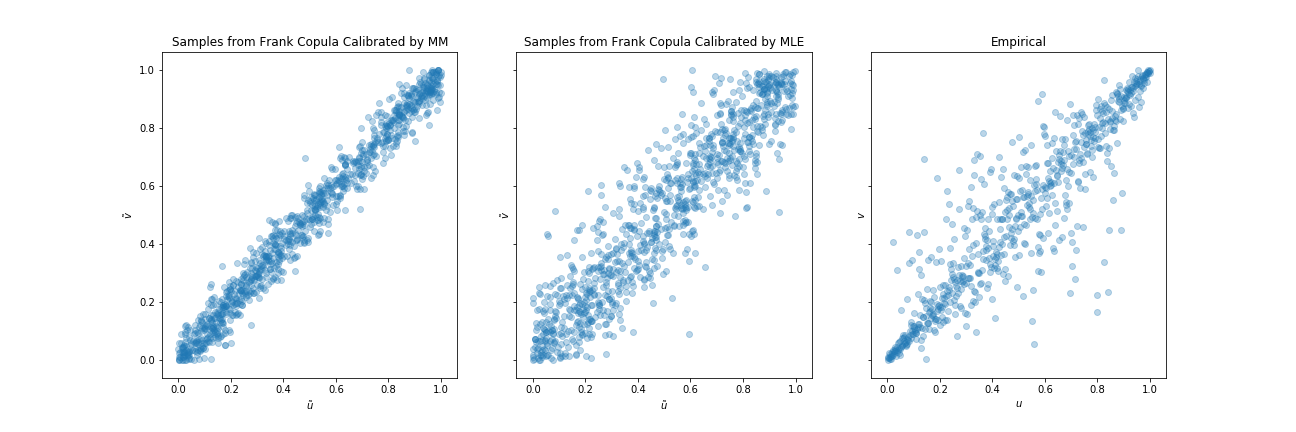
\includegraphics[width=\textwidth]{_pics/Frank.png}
   \caption{Comparison of Frank Copula Samples and Pseudo Observations of Bitcoin and CME Future Returns.
   }
   \label{fig:Frank}
\end{figure}

Aside from the Frank-copula, the HEs of various combination of copula and risk reduction objective are very similar.
This is an expected result as the portfolio consists only two assets.
In addition to hedging effectiveness, we observe the out-of-sample returns of the hedged portfolio.
Figure~\ref{fig:OOSRH} tabulates the time series of out-of-sample returns of hedged portfolio under various copulas and risk reduction objectives.

One can see all the combinations of copula and risk reduction objective generate a large fluctuation of returns in
25/09/2019 and 26/09/2019.
This large fluctuation is due to dependence break.
\medskip

\begin{figure}[th]
   \centering
   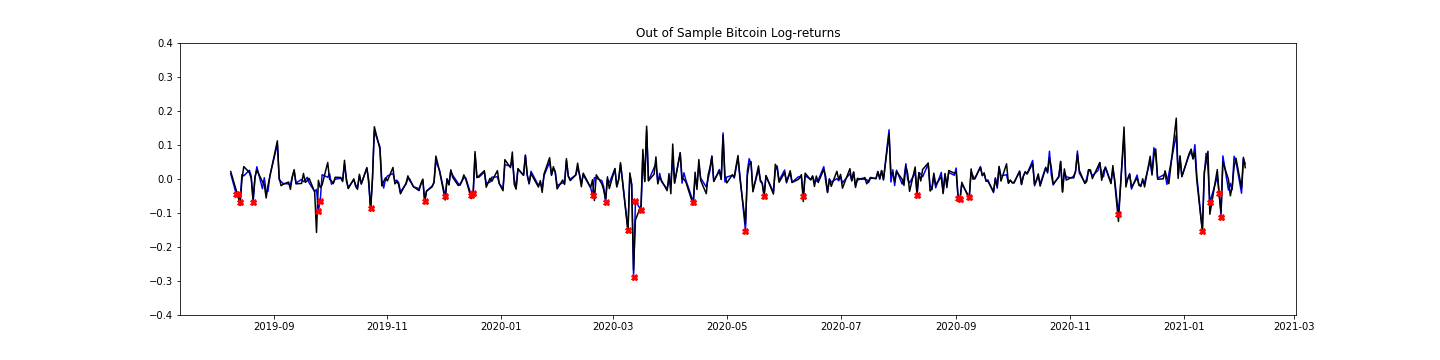
\includegraphics[width=\textwidth]{_pics/OOSBitcoin.png}
   \caption{Out of Sample Log-return of Bitcoin.
%   Lower Panel: Out of Sample Hedged Portfolio log-returns.
%   The $h^*$ is obtained from Gumbel copula aiming at reducing variance.
%   The red dots indicate the 30 most extreme negative returns in Bitcoin.
   }
   \label{fig:Gumbel}
\end{figure}

\newpage
\begin{landscape}
\begin{figure}[th]
   \centering
   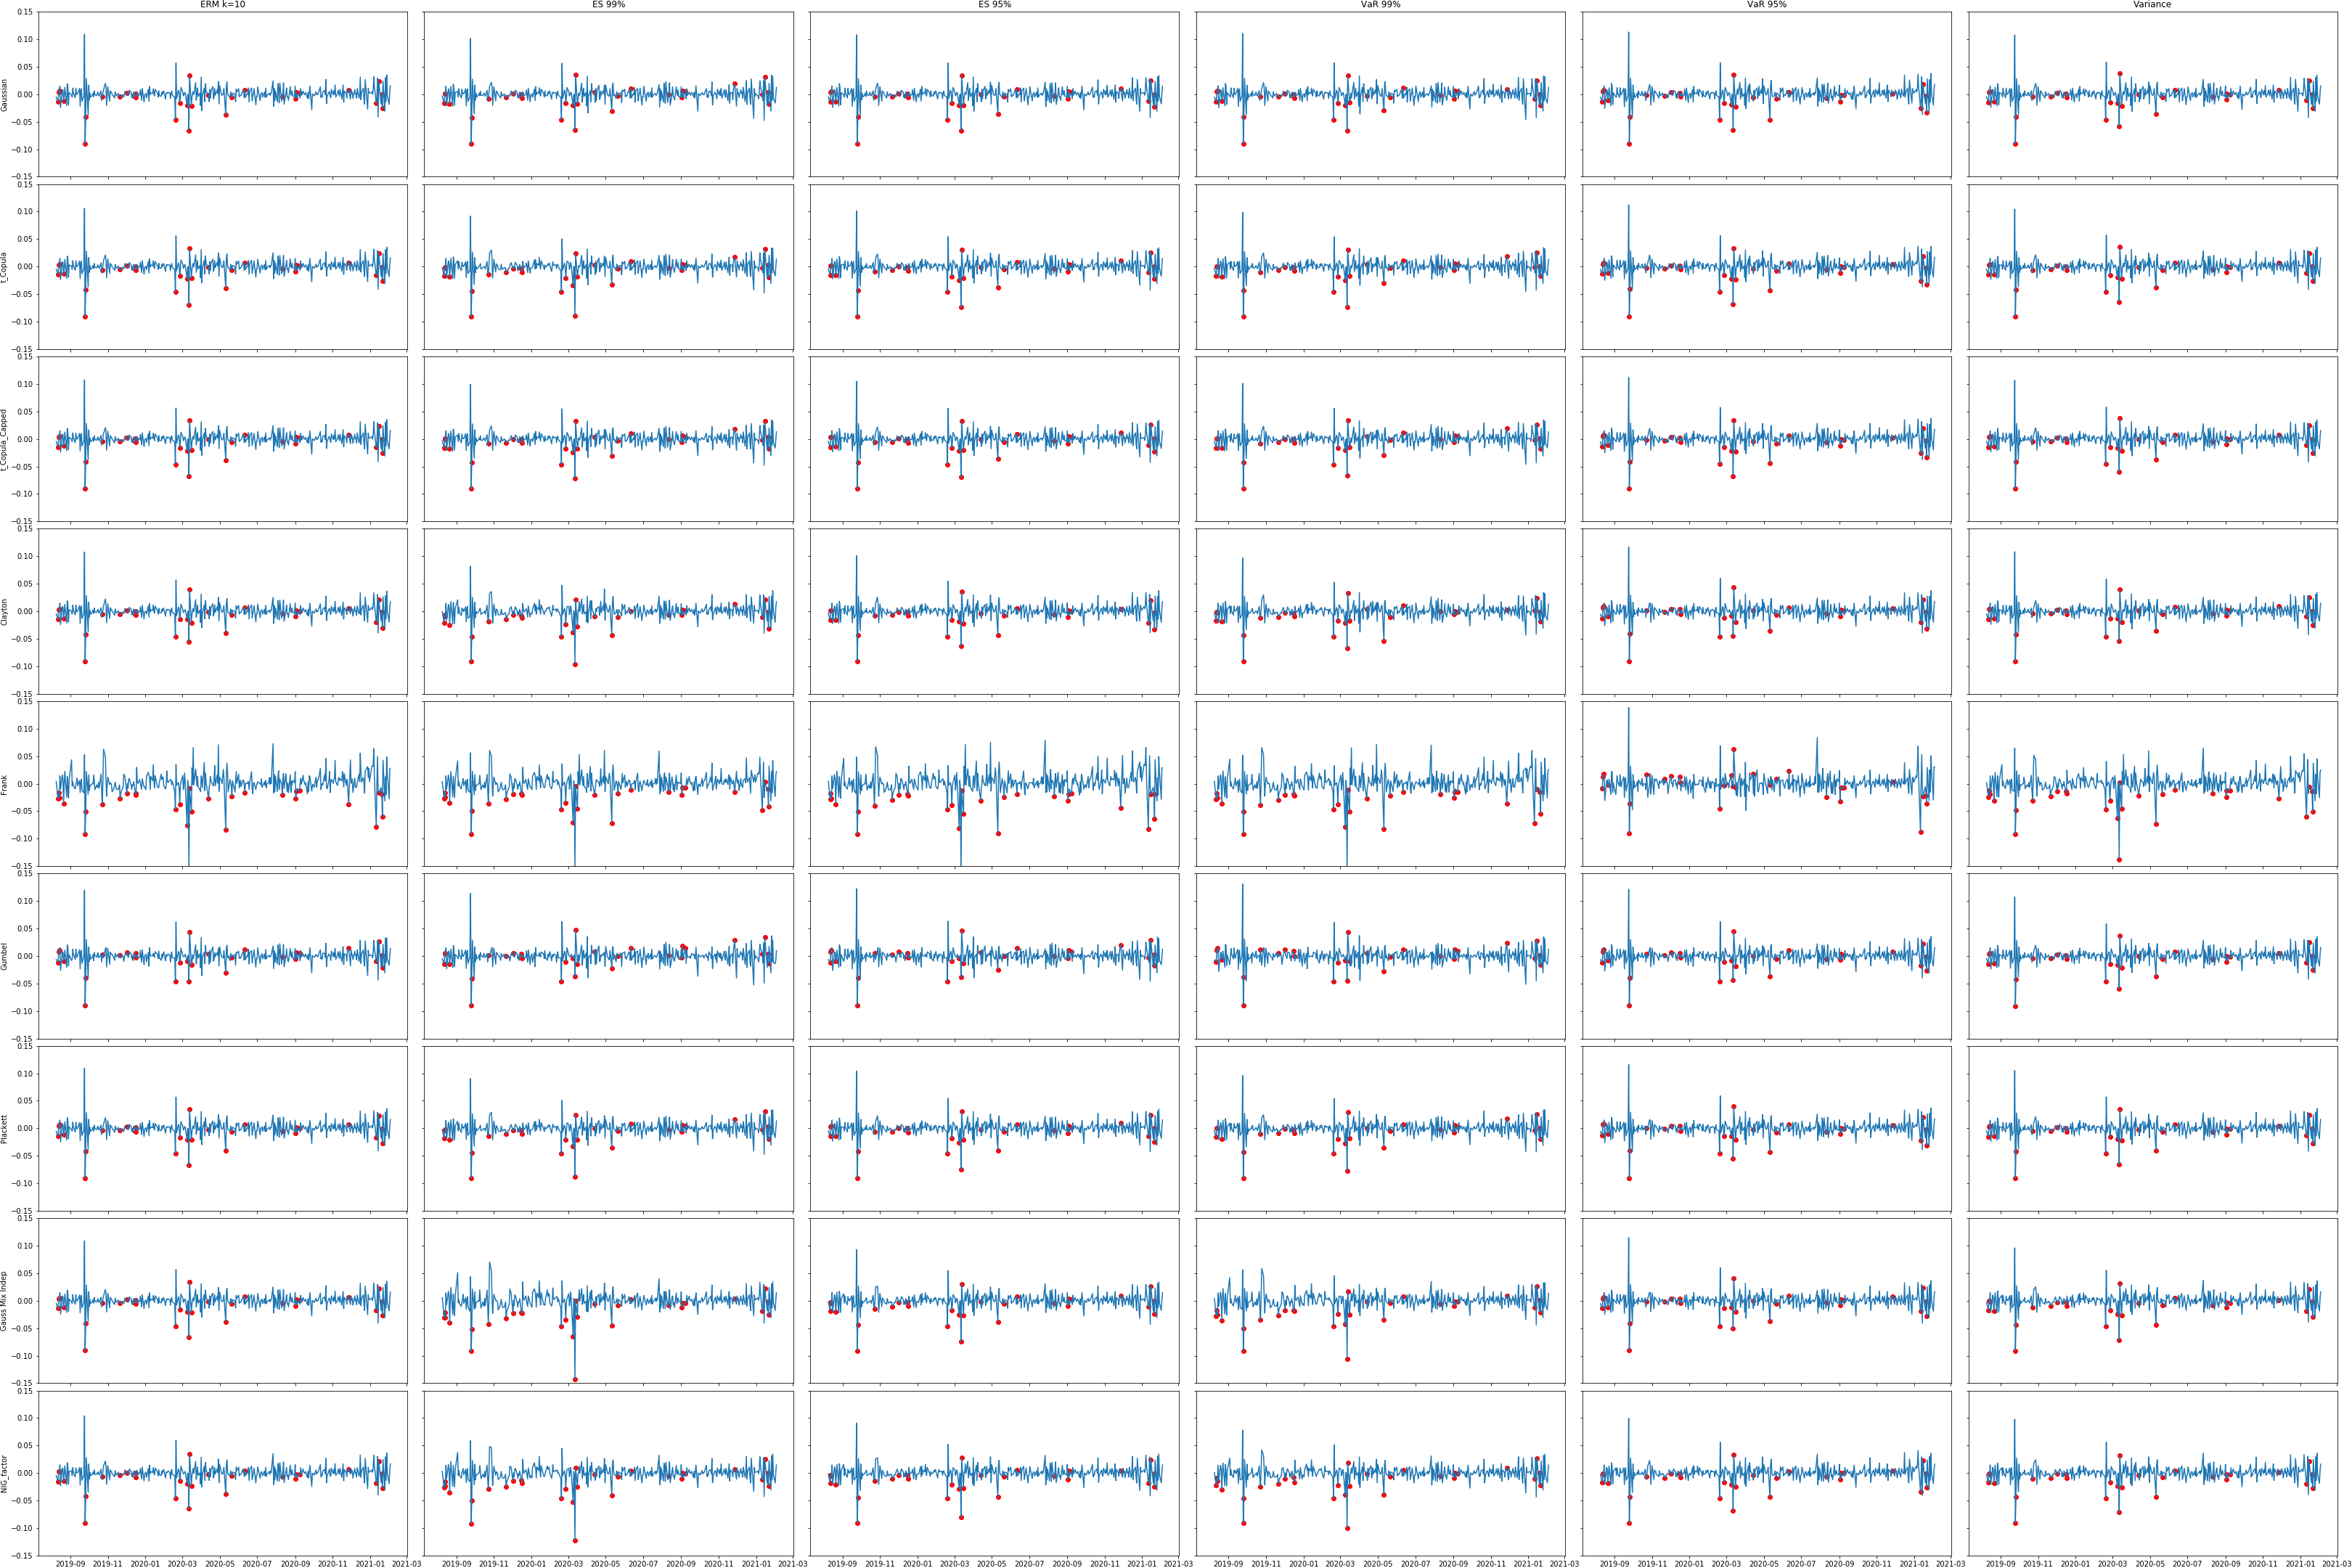
\includegraphics[width=\linewidth]{_pics/Rhs.png}
   \caption{Out-of-Sample Returns of Hedged Portfolio of Copulas and Risk Reduction Objectives.
   }
   \label{fig:OOSRH}
\end{figure}
\end{landscape}
\newpage

\newpage
\begin{landscape}
\begin{figure}[th]
   \centering
   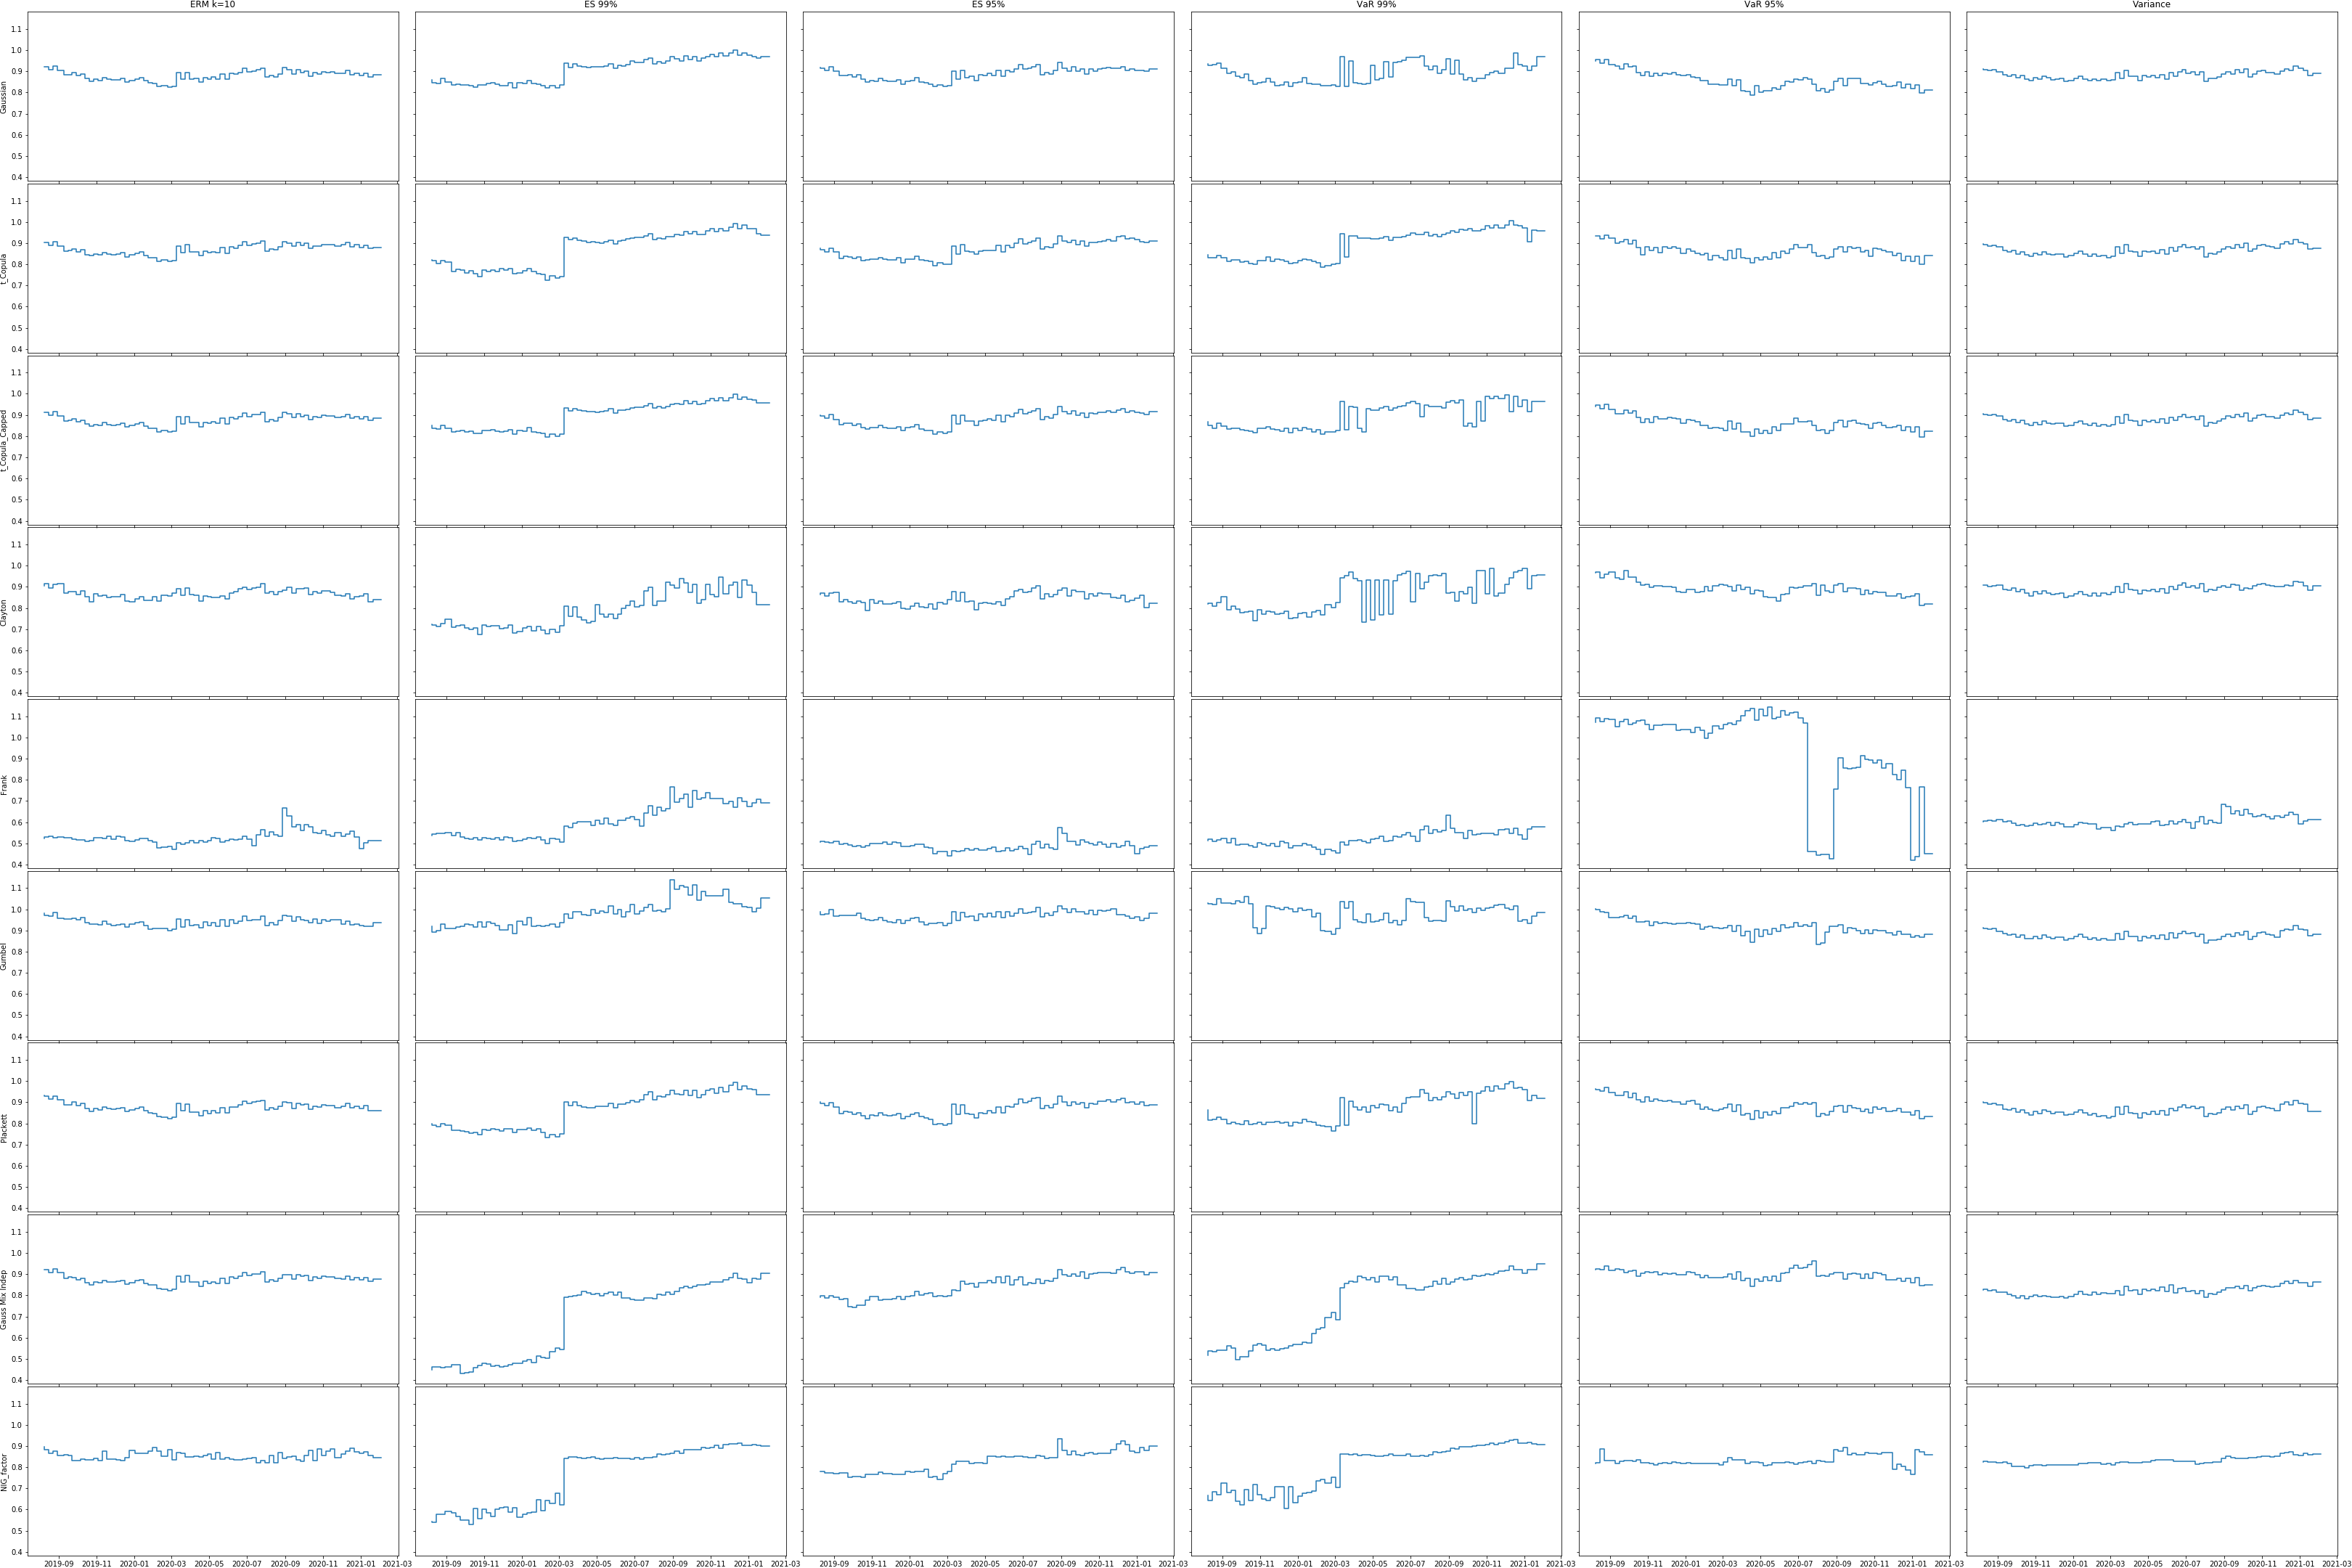
\includegraphics[width=\linewidth]{_pics/OHRs.png}
   \caption{Optimal Hedge Ratio Obtained from Combinations of Copula and Risk Reduction Objective.
   }
   \label{fig:OHRs}
\end{figure}
\end{landscape}
\newpage


%\begin{figure}[t]
%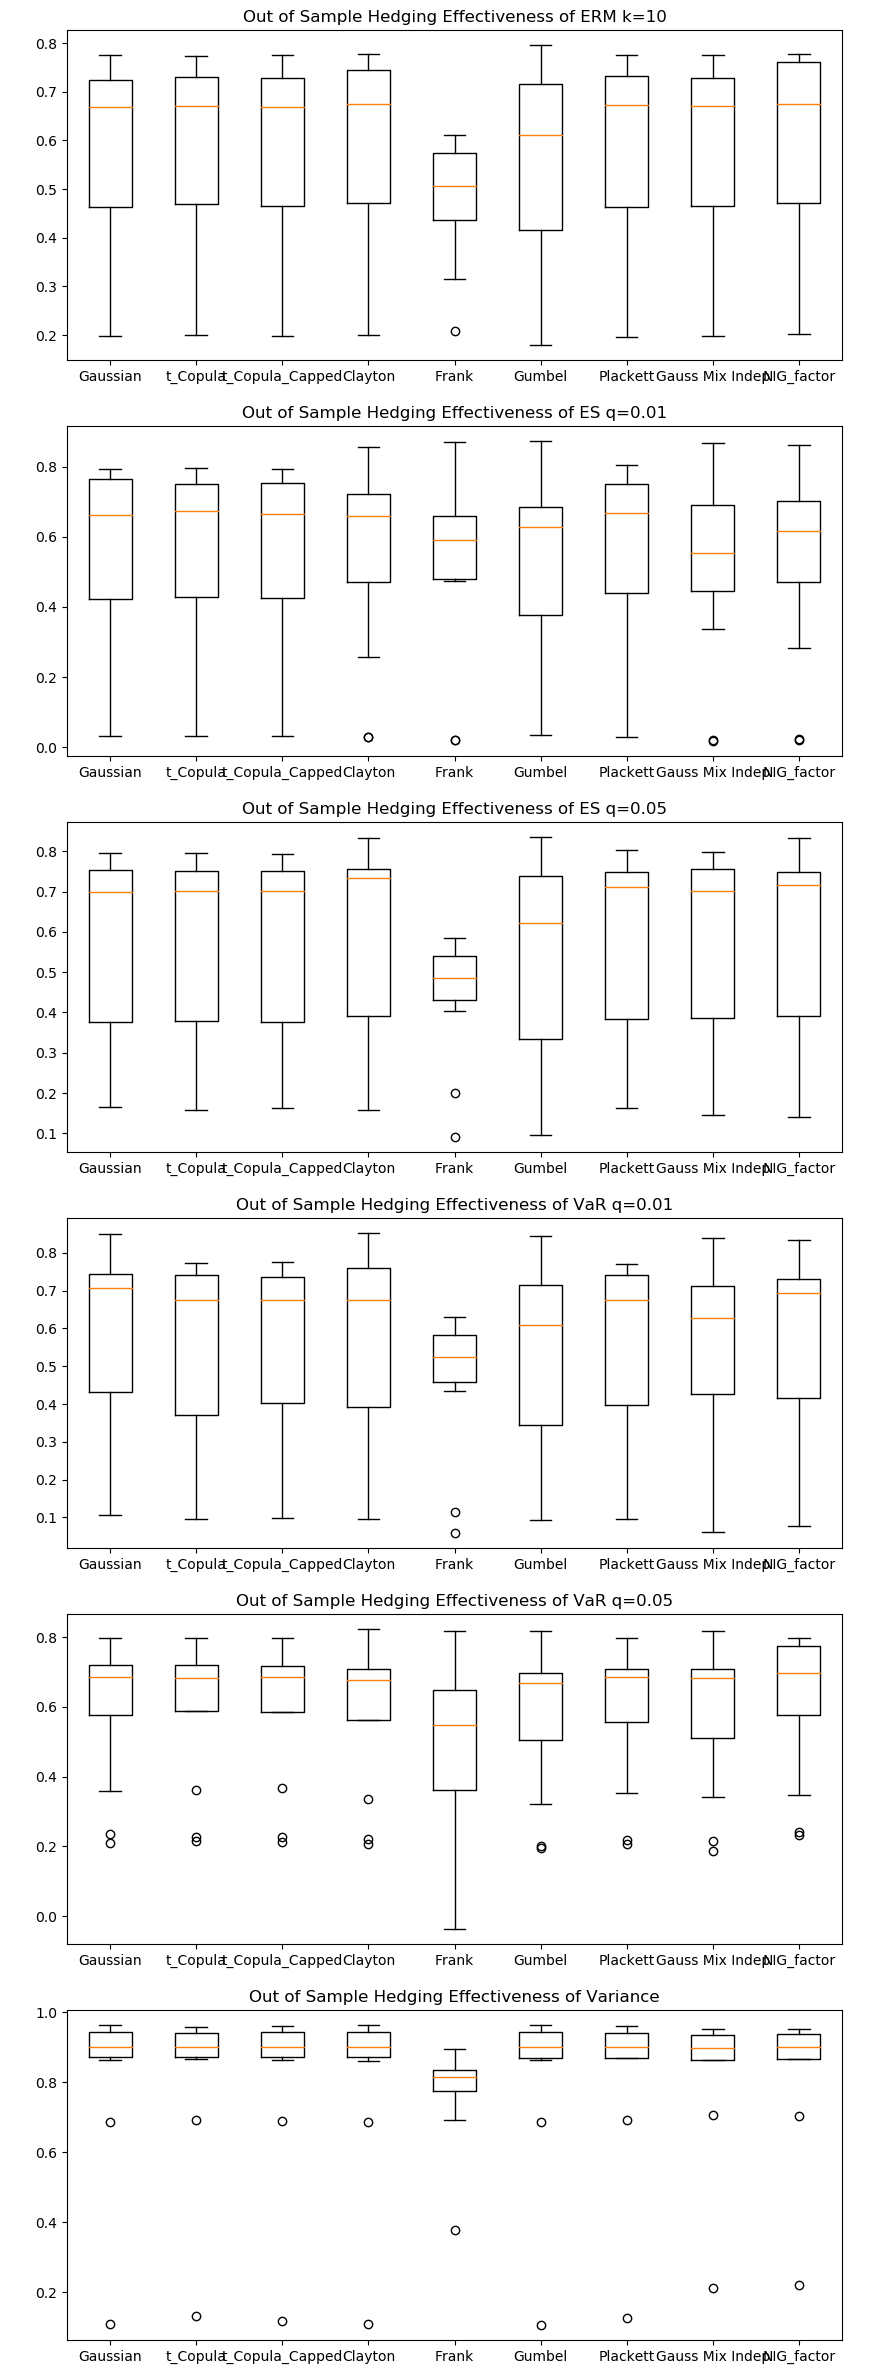
\includegraphics[width=\textwidth, height=\textheight]{_pics/Out of Sample Hedging Effectiveness.png}
%  \caption{}
%\label{out of Sample Hedging Effectieness}
%\end{figure}

\begin{figure}[!th]
   \centering
   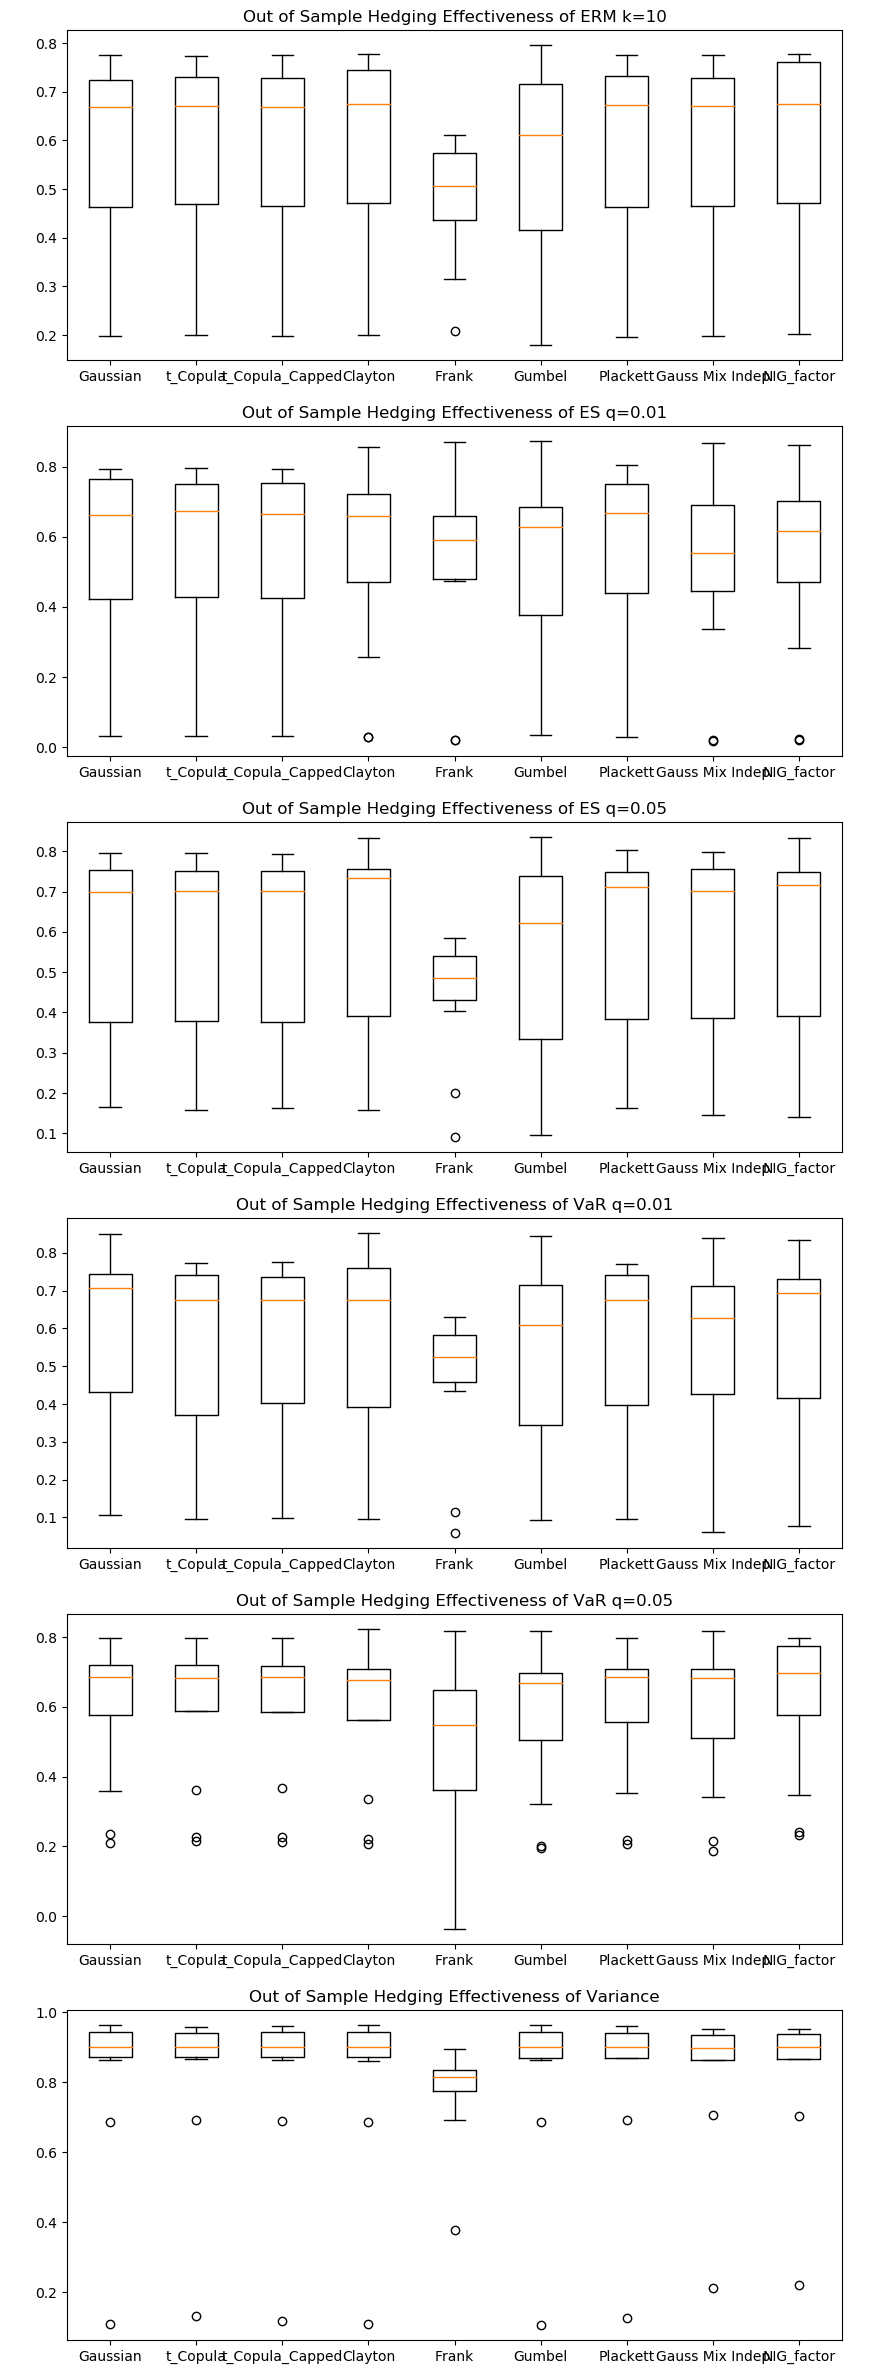
\includegraphics[height=25cm]{_pics/Out of Sample Hedging Effectiveness.png}
   \caption{Out of Sample Hedging Effectiveness Box-plot.
   The HEs are obtained from a set of out-of-sample data,
   each set consists 30 days log returns of Bitcoin and CME future.
   }
   \label{fig:OOSHE}
\end{figure}

Figure~\ref{fig:Gumbel} shows the time series of out-of-sample $R^h$ using Gumbel copula with the
objective of reducing variance.
The red dots are the 30 most extreme negative returns in Bitcoin.
In the figure, we can see the downside risk of Bitcoin is well managed by the hedging procedure with Gumbel copula.
Most of the extreme losses of Bitcoin are greatly reduced by introducing the CME future in the hedged portfolio.
Two exceptions are found in 25/09/2019 and 26/09/2019, where the CME future failed to follow the large drop in Bitcoin. (TODO: drop reason)
One of the possible reason is that traders was performing rollover activities on 25-26/09/2019, which
27/09/2019 is the expiry day of the September future.
Another reason for Gumbel fail of capturing the loss is dependence break.
The Kendall's tau in the training data is 0.2 higher than that of the testing data.
Other copulas suffer from the break as well.



\subsection{Stability of $h^*$}
We measure the stability of $h^*$ by sum of absolute change
\begin{align}
    \sum_{t=1}^T|h_t - h_{t-1}|.
    \end{align}

Adjustment of portfolio weights induces price slippage (ref) and transaction cost.
From figure \ref{SAD} we know the NIG factor copula with variance as risk reduction objective generates the smallest
sum of absolute change in OHR.

\begin{figure}[!th]
   \centering
   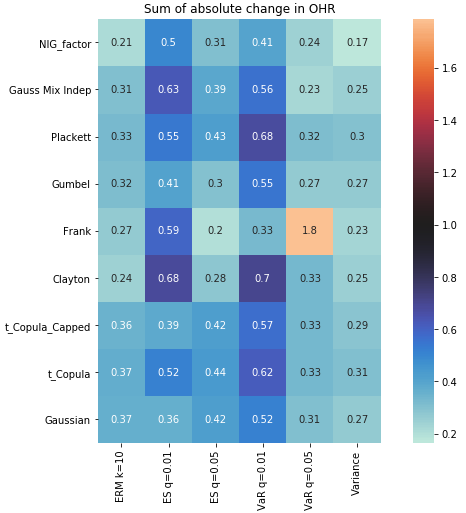
\includegraphics[width=\textwidth]{_pics/Sum of absolute change in OHR.png}
   \caption{Sum of Absolute Change in OHR.
   }
   \label{fig:SAD}
\end{figure}

%\usepackage{fontspec}
%\newcommand{\smallest}[1]{\textcolor{Maroon}{\textbf{#1}}}

\begin{table}
\begin{tabular}{lrrrrrr}
\toprule
{} &  ERM k=10 &    ES 99\% &    ES 95\% &   VaR 99\% &   VaR 95\% &  Variance \\
\midrule
Gaussian        &  0.019985 &  0.020802 &  0.020061 &  0.020230 &  0.019983 &  \color{blue}0.019757 \\
t\_Copula        &  0.020097 &  0.021698 &  0.020381 &  0.020966 &  0.020071 &  \color{blue}0.019890 \\
t\_Copula\_Capped &  0.020048 &  0.021018 &  0.020202 &  0.020554 &  0.020059 &  \color{blue}0.019792 \\
Clayton         &  0.019519 &  0.021341 &  0.019789 &  0.021045 &  \color{blue}0.019389 &  0.019675 \\
Frank           &  0.029234 &  0.026240 &  0.030770 &  0.029157 &  \color{blue}0.023085 &  0.025928 \\
Gumbel          &  0.020014 &  0.021411 &  0.020511 &  0.021643 &  \color{blue}0.019557 &  0.019757 \\
Plackett        &  0.020010 &  0.021531 &  0.020363 &  0.020870 &  \color{blue}0.019755 &  0.019909 \\
Gauss Mix Indep &  0.019949 &  0.025390 &  0.020454 &  0.023283 &  \color{blue}0.019667 &  0.020006 \\
NIG\_factor      &  \color{blue}0.019720 &  0.023425 &  0.020706 &  0.022039 &  0.019950 &  0.019999 \\
\bottomrule
\end{tabular}
\caption{Exponential Risk Measure $k=10$}
\end{table}

\begin{table}
\begin{tabular}{lrrrrrr}
\toprule
{} &  ERM k=10 &    ES 99\% &    ES 95\% &   VaR 99\% &   VaR 95\% &  Variance \\
\midrule
Gaussian        &  0.061084 &  0.062405 &  0.061201 &  0.062148 &  0.061712 &  \color{blue}0.059310 \\
t\_Copula        &  0.062148 &  0.068702 &  0.063339 &  0.063964 &  0.062067 & \color{blue}0.060735 \\
t\_Copula\_Capped &  0.061623 &  0.064114 &  0.062198 &  0.062466 &  0.062072 & \color{blue}0.059676 \\
Clayton         &  0.058495 &  0.069910 &  0.060812 &  0.064595 &  \color{blue}0.055962 &  0.058318 \\
Frank           &  0.104185 &  0.096795 &  0.108713 &  0.105070 &  \color{blue}0.068457 &  0.091321 \\
Gumbel          &  0.056513 &  0.059574 &  0.056035 &  0.058162 &  \color{blue}0.055492 &  0.059525 \\
Plackett        &  0.061167 &  0.068027 &  0.063426 &  0.064563 &  \color{blue}0.058491 &  0.061017 \\
Gauss Mix Indep &  0.061157 &  0.088023 &  0.063900 &  0.073316 &  \color{blue}0.057007 &  0.063081 \\
NIG\_factor      &  \color{blue}0.060878 &  0.078959 &  0.065270 &  0.070919 &  0.062097 &  0.062848 \\
\bottomrule
\end{tabular}
\caption{ES 99\%}
\end{table}

\begin{table}
\begin{tabular}{lrrrrrr}
\toprule
{} &  ERM k=10 &    ES 99\% &    ES 95\% &   VaR 99\% &   VaR 95\% &  Variance \\
\midrule
Gaussian        &  0.034488 &  0.035237 &  0.034548 &  0.035123 &  0.034838 &  \color{blue}0.034248 \\
t\_Copula        &  0.034777 &  0.037100 &  0.035234 &  0.035634 &  0.035055 &  \color{blue}0.034494 \\
t\_Copula\_Capped &  0.034647 &  0.035679 &  0.034862 &  0.035282 &  0.034937 &  \color{blue}0.034322 \\
Clayton         &  0.033714 &  0.037282 &  0.034230 &  0.036089 &  \color{blue}0.033445 &  0.034046 \\
Frank           &  0.053661 &  0.047849 &  0.056299 &  0.053409 &  \color{blue}0.037638 &  0.046953 \\
Gumbel          &  0.034028 &  0.035965 &  0.034528 &  0.036353 &  \color{blue}0.033568 &  0.034293 \\
Plackett        &  0.034592 &  0.036831 &  0.035316 &  0.035752 &  \color{blue}0.034186 &  0.034558 \\
Gauss Mix Indep &  0.034439 &  0.045160 &  0.035120 &  0.040027 &  \color{blue}0.033756 &  0.034478 \\
NIG\_factor      &  \color{blue}0.033882 &  0.041001 &  0.035677 &  0.037975 &  0.034656 &  0.034453 \\
\bottomrule
\end{tabular}
\caption{ES 95\%}
\end{table}

\begin{table}
\begin{tabular}{lrrrrrr}
\toprule
{} &  ERM k=10 &    ES 99\% &    ES 95\% &   VaR 99\% &   VaR 95\% &  Variance \\
\midrule
Gaussian        &  \color{blue}0.041327 &  0.044416 &  0.041943 &  0.043399 &  0.042275 &  0.041981 \\
t\_Copula        &  \color{blue}0.041450 &  0.044830 &  0.042806 &  0.043789 &  0.041693 &  0.041969 \\
t\_Copula\_Capped &  \color{blue}0.041498 &  0.044169 &  0.042411 &  0.044051 &  0.042018 &  0.042056 \\
Clayton         &  \color{blue}0.040022 &  0.044523 &  0.042878 &  0.044215 &  0.040913 &  0.041943 \\
Frank           &  0.076644 &  0.055387 &  0.081273 &  0.073433 &  \color{blue}0.046177 &  0.061056 \\
Gumbel          &  0.042079 &  0.042139 &  0.042187 &  0.045340 &  \color{blue}0.040523 &  0.041937 \\
Plackett        &  \color{blue}0.041013 &  0.044971 &  0.042370 &  0.042995 &  0.041574 &  0.041731 \\
Gauss Mix Indep &  0.040998 &  0.048017 &  0.043249 &  0.044518 &  \color{blue}0.040749 &  0.043386 \\
NIG\_factor      &  \color{blue}0.040457 &  0.047201 &  0.043925 &  0.044230 &  0.043240 &  0.043138 \\
\bottomrule
\end{tabular}
\caption{VaR 99\%}
\end{table}

\begin{table}
\begin{tabular}{lrrrrrr}
\toprule
{} &  ERM k=10 &    ES 99\% &    ES 95\% &   VaR 99\% &   VaR 95\% &  Variance \\
\midrule
Gaussian        &  0.020385 &  0.020315 &  0.020143 &  0.020412 &  0.020121 &  \color{blue}0.019579 \\
t\_Copula        &  0.020547 &  0.020428 &  0.020661 &  0.020611 &  0.020370 &  \color{blue}0.019820 \\
t\_Copula\_Capped &  0.020525 &  0.020544 &  0.020503 &  0.020486 &  0.020224 &  \color{blue}0.019656 \\
Clayton         &  0.019702 &  0.021042 &  0.020143 &  0.020640 &  0.019990 &  \color{blue}0.019700 \\
Frank           &  0.026372 &  0.023529 &  0.027105 &  0.026212 &  \color{blue}0.023389 &  0.023594 \\
Gumbel          &  0.019781 &  0.021311 &  0.020716 &  0.020421 &  \color{blue}0.019077 &  0.019541 \\
Plackett        &  0.020459 &  0.020257 &  0.020589 &  0.020100 &  0.020237 &  \color{blue}0.020047 \\
Gauss Mix Indep &  0.020482 &  0.024753 &  0.020304 &  0.024158 &  \color{blue}0.019944 &  0.020723 \\
NIG\_factor      &  \color{blue}0.019923 &  0.023784 &  0.021009 &  0.022172 &  0.019980 &  0.020670 \\
\bottomrule
\end{tabular}
\caption{VaR 95\%}
\end{table}

\begin{table}
\begin{tabular}{lrrrrrr}
\toprule
{} &  ERM k=10 &    ES 99\% &    ES 95\% &   VaR 99\% &   VaR 95\% &  Variance \\
\midrule
Gaussian        &  0.014387 &  0.014380 &  0.014360 &  0.014530 &  0.014670 &  \color{blue}0.014294 \\
t\_Copula        &  0.014378 &  0.014626 &  0.014343 &  0.014385 &  0.014627 &  \color{blue}0.014306 \\
t\_Copula\_Capped &  0.014375 &  0.014418 &  0.014332 &  0.014430 &  0.014643 &  \color{blue}0.014290 \\
Clayton         &  0.014306 &  0.014870 &  0.014332 &  0.014532 &  0.014493 &  \color{blue}0.014267 \\
Frank           &  0.021495 &  0.018982 &  0.022736 &  0.021476 &  \color{blue}0.018142 &  0.018897 \\
Gumbel          &  0.014618 &  0.014971 &  0.014878 &  0.015438 &  0.014622 &  \color{blue}0.014321 \\
Plackett        &  0.014444 &  0.014560 &  0.014424 &  0.014423 &  0.014596 &  \color{blue}0.014353 \\
Gauss Mix Indep &  0.014404 &  0.017404 &  \color{blue}0.014341 &  0.015671 &  0.014453 &  0.014408 \\
NIG\_factor      &  \color{blue}0.014362 &  0.015841 &  0.014484 &  0.015043 &  0.014474 &  0.014415 \\
\bottomrule
\end{tabular}
\caption{Standard Deviation}
\end{table}
% ----------------
% --- Results ---
% ----------------

\newpage
%
\bibliography{finance} %
\newpage
\section{Appendix}\label{sec:appendix}

\begin{proposition}
   Let $\bm{X} = (X_1, ..., X_d)^\top$ be real-valued random variables with corresponding
   copula density $\bm{c}_{X_1, ..., X_d}$, and continuous marginals $F_{X_1}, ..., F_{X_d}$.
   Then,
   density of the linear combination of marginals $Z = n_1 \cdot X_1 + ... +  n_d \cdot X_d $ is

   \begin{align}
   f_Z(z) &= \left| n_1^{-1} \right| \int_{[0,1]^{d-1}} \left[ \bm{c}_{X_1,...,X_d}
      \{F_{X_1} \circ S(z), u_2, ..., u_d \} \cdot
      f_{X_1} \circ S(z) \right] du_2 ... du_d \label{density} \\
      S(z) &= \frac{1}{n_1}\cdot z - \frac{n_2}{n_1} \cdot F^{-1}_{X_2}(u_2) - ... -  \frac{n_d}{n_1} \cdot F^{-1}_{X_d}(u_d)
      \end{align}
   \end{proposition}

\begin{proof} \medskip
   Rewrite $Z = n_1 \cdot X_1 + ... +  n_d \cdot X_d $ in matrix form
   \begin{align}
      \begin{bmatrix}
      Y \\ X_2 \\ \vdots \\ X_d
      \end{bmatrix}
      = \begin{bmatrix}
      n_1    & n_2   & \cdots & n_d     \\
      0      & 1     &  \cdots & 0       \\
      \vdots &       & \ddots & \vdots \\
      0      & \cdots &       & 1  \\
      \end{bmatrix}
      \begin{bmatrix}
         X_1 \\ X_2 \\ \vdots \\ X_d
      \end{bmatrix}
      = \bm{A}
      \begin{bmatrix}
         X_1 \\ X_2 \\ \vdots \\ X_d
      \end{bmatrix}.
      \end{align} \medskip

   By transformation variables
   \begin{align}
      \bm{f}_{Z,X_2,...,X_d}(z, x_2, ...,x_d) &= \bm{f}_{X_1,...,X_d}\left( \bm{A}^{-1}
      \begin{bmatrix}
         z \\ x_2 \\ \vdots \\ x_d
      \end{bmatrix}
      \right)  \cdot |\det \bm{A}^{-1}| \\
      &= \left| n_1^{-1} \right| \bm{f}_{X_1,...,X_d}\{S(z), x_2,...,x_d\}
      \end{align} \medskip

   Let $u_i = F_{X_i}(x_i)$ and
   use the relationship
   \begin{align}
      \bm{c}_{X_1,...,X_d}(u_1, ..., u_d)=\frac{\bm{f}_{X_1,...,X_d}(x_1,...,x_d)}{\prod_{i=1}^d f_{X_i}(x_i)},
   \end{align}
   we have
   \begin{align}
     & \bm{f}_{Z,X_2,...,X_d}(z, x_2, ...,x_d) = \\
      & \left| n_1^{-1} \right| \cdot
      \bm{c}_{X_1,...,X_d}\{F_{X_1} \circ S(z), u_2, ...,  u_d\}  \cdot
      f_{X_1} \{ S(z) \} \cdot
      \prod_{i=2}^d f_{X_i}(x_i)
      \end{align}

   The claim \ref{density} is obtained by integrating out $x_2, ... x_d$ by substituting $dx_i = \frac{1}{f_{X_i}(x_i)}du_i$.
   \end{proof}
\end{document}
